\chapter{依赖关系的度量}
\label{chap:dependence-measures}

在区间$[-1,1]$上均匀地取一个数$X$，再令$Y=X^{2}$。知道$X$就完全知道$Y$，两个变量之间的联系再紧密不过；可是它们的协方差恰好为零。若只拿相关系数去判断，会得出“两者没有关系”的结论。问题出在相关系数只检查一种特定的联系：$Y$是否随$X$线性地增减。抛物线左半支下降、右半支上升，两种趋势正好抵消。

要回答“$X$与$Y$是否独立”，需要比较整个联合分布$P_{(X,Y)}$与边缘乘积$P_X\otimes P_Y$。两者相等就是独立；不等时，差别可以从多个角度去量：观测一个变量后另一个变量的不确定性减少了多少，成对距离是否一起变化，联合分布与边缘乘积在某个核空间里相距多远，把取值装进有限个格子后格子标签之间是否还有关联。每个角度给出一个依赖度量，它们的零值、取值范围、对坐标变换的反应和需要的参数各不相同。

第一节用抛物线和几个零相关的例子把共同问题提出来，区分三件事：零值能否刻画独立，非零数值怎样随依赖变化，以及能否从有限样本可靠地判断。后面四节依次研究四类度量。互信息直接回用第~\ref{chap:information-measures}章的定义，这里关心它对一一变换的不变性，以及确定关系为什么给出无穷大。距离协方差用特征函数之差的加权积分定义，它能写成成对距离的期望，归一化后得到距离相关。HSIC把联合分布与边缘乘积放进乘积核的RKHS，用第~\ref{chap:distribution-comparison}章的MMD比较。离散化评分先把取值分格，再对格子标签计算互信息。最后一节把这些量放在同一组分布上比较。

全章贯穿三个例子：三点抛物线（$X$在$\{-1,0,1\}$上等可能，$Y=X^{2}$），连续抛物线（$X\sim\operatorname{Unif}(-1,1)$，$Y=X^{2}$，必要时加噪声），以及相关系数为$\rho$的标准二元高斯分布。本章讨论的都是给定联合分布时的总体量；由样本估计这些量、校准估计误差和检验独立性，属于统计推断的问题。

\section{从相关到独立}
\label{sec:dep-correlation-to-independence}

协方差为零时，两个变量还可能有多强的联系？先把开头的抛物线算清楚。

\paragraph{零协方差的抛物线}
设$X\sim\operatorname{Unif}(-1,1)$，$Y=X^{2}$。$X$的密度在$[-1,1]$上为$1/2$，奇数次矩为零，于是
\[
  \mathbb{E}[X]=0,\qquad \mathbb{E}[X^{3}]=\frac12\int_{-1}^{1}x^{3}\,\mathrm{d}x=0 .
\]
代入协方差的定义，得到
\[
  \operatorname{Cov}(X,Y)=\mathbb{E}[XY]-\mathbb{E}[X]\,\mathbb{E}[Y]=\mathbb{E}[X^{3}]-0=0 .
\]
$X$与$Y$不相关。但它们并不独立：事件$A=\{\lvert X\rvert\leq1/2\}$发生时一定有$Y\leq1/4$，所以
\[
  \mathbb{P}\bigl(\lvert X\rvert\leq\tfrac12,\ Y>\tfrac14\bigr)=0 .
\]
若两者独立，这个概率应当等于两个边缘概率的乘积，
\[
  \mathbb{P}\bigl(\lvert X\rvert\leq\tfrac12\bigr)\,\mathbb{P}\bigl(Y>\tfrac14\bigr)=\frac12\cdot\frac12=\frac14 .
\]

图~\ref{fig:dep-parabola-joint-product}把这两个数画了出来。左图是$(X,Y)$的样本，全部落在抛物线上；右图是“假装独立”的样本：$X$与$Y$各按自己的边缘分布抽取，但彼此独立。两幅图的横坐标分布相同，纵坐标分布也相同，差别只在点怎样配对。红框里的事件在左图中没有点，在右图中约占四分之一。

\begin{BookInlineFigure}
  \centering
  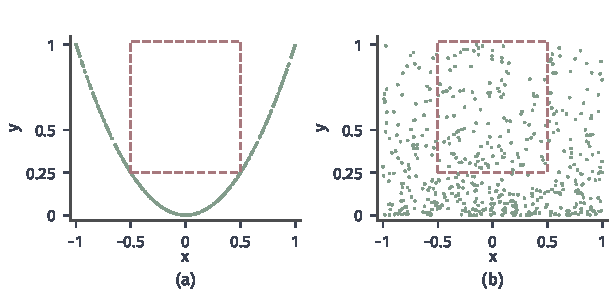
\includegraphics[width=104mm]{figures/07-probability/04-distribution-analysis/matplotlib/dep-parabola-joint-product/figure.pdf}
  \caption{同样的边缘，不同的配对。(a)$X\sim\operatorname{Unif}(-1,1)$，$Y=X^{2}$的$500$个样本（绿）；(b)边缘乘积$P_X\otimes P_Y$的$500$个样本，即把$X$与一个独立复制$X'$的平方配对。红色虚线框是事件$\{\lvert x\rvert\leq1/2,\ y>1/4\}$，其概率在(a)中为$0$，在(b)中为$1/4$（样本中占$0.248$）。种子$719$。}
  \label{fig:dep-parabola-joint-product}
\end{BookInlineFigure}

\paragraph{协方差只是一个测试}
协方差为零说的是$\mathbb{E}[(X-\mathbb{E}X)(Y-\mathbb{E}Y)]=0$，即一对特定函数$x\mapsto x$、$y\mapsto y$的乘积在联合分布下的期望，与在边缘乘积下的期望相同。独立要求的多得多：对一切有界可测函数$f,g$，
\begin{equation}
  \mathbb{E}\bigl[f(X)\,g(Y)\bigr]=\mathbb{E}\bigl[f(X)\bigr]\,\mathbb{E}\bigl[g(Y)\bigr],
  \label{eq:dep-independence-test-functions}
\end{equation}
这等价于联合分布等于边缘乘积，
\begin{equation}
  P_{(X,Y)}=P_X\otimes P_Y .
  \label{eq:dep-independence}
\end{equation}
取$f,g$为示性函数，式~\eqref{eq:dep-independence-test-functions}就是矩形事件上的乘积公式，它确定两个分布相等；反过来，由矩形事件的乘积公式经简单函数逼近得到一般有界$f,g$的情形，这正是第~\ref{chap:probability-spaces}章建立独立性时走过的路。

协方差是式~\eqref{eq:dep-independence-test-functions}中只取一对线性函数的结果，换一对函数就能看出抛物线的依赖。取$f(x)=x^{2}$，$g(y)=y$，由$\mathbb{E}[X^{2}]=1/3$与$\mathbb{E}[X^{4}]=1/5$，
\[
  \operatorname{Cov}\bigl(X^{2},Y\bigr)=\operatorname{Var}\bigl(X^{2}\bigr)=\frac15-\frac19=\frac{4}{45}>0 .
\]
所以“协方差为零”只排除了一种线性的联系。这一点在第~\ref{chap:random-vectors}章已经见过：不相关不等于独立。

\paragraph{零相关的几种形状}
图~\ref{fig:dep-zero-correlation-shapes}收集了几种协方差为零的联合分布。(b)中$Y=SX$，$S$是与$X$独立、等可能取$\pm1$的随机符号，协方差是$\mathbb{E}[S]\,\mathbb{E}[X^{2}]=0$，可是$\lvert Y\rvert=\lvert X\rvert$。(c)是单位圆周上的均匀分布，两个坐标满足$X^{2}+Y^{2}=1$。只有(d)两个坐标独立。四幅图的相关系数都是零，相关系数无法把(d)与前三幅区分开。

\begin{BookInlineFigure}
  \centering
  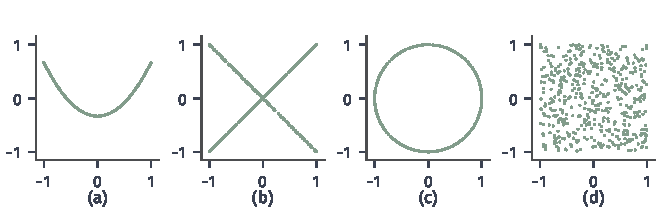
\includegraphics[width=112mm]{figures/07-probability/04-distribution-analysis/matplotlib/dep-zero-correlation-shapes/figure.pdf}
  \caption{协方差都为零的四个联合分布，各$500$个样本（种子$719$）。(a)$X\sim\operatorname{Unif}(-1,1)$与$X^{2}-1/3$；(b)$X$与$SX$，$S$为独立随机符号；(c)单位圆周上的均匀分布；(d)两个独立的$\operatorname{Unif}(-1,1)$。前三个都不独立。}
  \label{fig:dep-zero-correlation-shapes}
\end{BookInlineFigure}

\paragraph{相关足够的两种情形}
有两类联合分布，零相关确实等价于独立。一类是联合高斯向量，第~\ref{chap:multivariate-distributions}章已经证明。另一类是两个二值变量。设$X,Y$都取值于$\{0,1\}$，记$p=\mathbb{P}(X=1)$，$q=\mathbb{P}(Y=1)$。由$XY=\mathbf{1}_{\{X=1,Y=1\}}$，
\[
  \mathbb{P}(X=1,\,Y=1)-pq=\mathbb{E}[XY]-\mathbb{E}[X]\,\mathbb{E}[Y]=\operatorname{Cov}(X,Y).
\]
其余三个格子由边缘减出来。例如$\mathbb{P}(X=1,Y=0)=p-\mathbb{P}(X=1,Y=1)$，它与$p(1-q)$之差是$-\operatorname{Cov}(X,Y)$。所以$2\times2$概率表的四个格子与独立时的乘积只差$\pm\operatorname{Cov}(X,Y)$，协方差为零时四个格子都分解成乘积。二值变量只有一个“自由度”可以偏离独立，协方差恰好量的就是它。取值多于两个时，偏离独立的方向不止一个，单个协方差看不全。

\paragraph{三点抛物线}
最小的反例只需要三个点。设$X$在$\{-1,0,1\}$上等可能，$Y=X^{2}$。$(X,Y)$等可能取$(-1,1)$、$(0,0)$、$(1,1)$三个值，边缘为
\[
  \mathbb{P}(X=x)=\tfrac13\ (x=-1,0,1),\qquad \mathbb{P}(Y=1)=\tfrac23,\qquad \mathbb{P}(Y=0)=\tfrac13 .
\]
协方差仍是$\mathbb{E}[X^{3}]=\frac13(-1+0+1)=0$。图~\ref{fig:dep-three-point-tables}把联合概率表与边缘乘积表并排放在一起：联合表有三个格子为零，乘积表六个格子都是正数。这个例子取值有限，所有度量都能手算，后面每一节都会回到它。

\begin{BookInlineFigure}
  \centering
  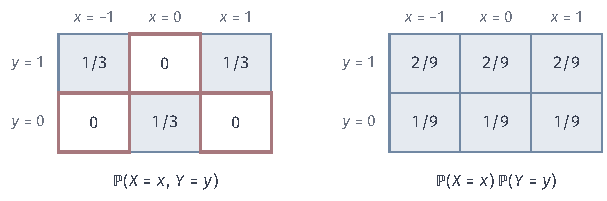
\includegraphics[width=102.8mm]{figures/07-probability/04-distribution-analysis/tikz/dep-three-point-tables/figure.pdf}
  \caption{三点抛物线。左：联合概率表$\mathbb{P}(X=x,Y=y)$，浅蓝格子有正质量，红框标出联合表为零而乘积表为正的三个格子。右：边缘乘积$\mathbb{P}(X=x)\,\mathbb{P}(Y=y)$，其中$\mathbb{P}(Y=1)=2/3$，$\mathbb{P}(Y=0)=1/3$。}
  \label{fig:dep-three-point-tables}
\end{BookInlineFigure}

\paragraph{依赖度量要回答的三件事}
于是共同的问题是：$P_{(X,Y)}$离$P_X\otimes P_Y$有多远。把联合分布映成一个非负数的泛函，称为\term{依赖度量}（dependence measure）。评价一个依赖度量，要把三件不同的事分开。

第一件是零值判据：度量为零是否当且仅当独立。协方差在一般分布上做不到，在联合高斯和二值变量上做得到；本章的互信息、距离协方差、高斯核HSIC在各自的条件下都做得到。第二件是非零数值的含义：依赖变强时数值是否增大，有没有上界，对重新标记、平移、缩放、单调变换是否敏感，需要预先选哪些参数。这一件没有统一答案，不同度量给同一对分布排出的强弱次序可以相反。第三件是有限样本：只观测到$n$对数据时，能否可靠地判断度量是否为零，误差有多大。

本章的定义都是总体量，只回答前两件事。第三件要另外分析估计量的偏差、方差和分布，即使度量的零值完全刻画独立，样本上算出的一个正数也不等于证明了依赖，这部分由统计推断承担，可参考\BookChapterRef{chap:nonparametric-inference}{卷八第2章“非参数分布与函数推断”}。


\section{互信息作为依赖量}
\label{sec:dep-mutual-information}

第~\ref{chap:information-measures}章已经给出一个直接比较式~\eqref{eq:dep-independence}两边的量。设$X,Y$分别取值于可测空间$\mathcal{X},\mathcal{Y}$，互信息定义为联合分布相对边缘乘积的KL散度，
\begin{equation}
  I(X;Y)=D_{\mathrm{KL}}\bigl(P_{(X,Y)}\,\Vert\,P_X\otimes P_Y\bigr)\in[0,\infty].
  \label{eq:dep-mi}
\end{equation}
按第~\ref{chap:distribution-comparison}章的约定，若$P_{(X,Y)}$不绝对连续于$P_X\otimes P_Y$，KL散度取$+\infty$。那里也证明了KL散度非负、且为零当且仅当两个分布相同，所以
\[
  I(X;Y)=0\iff P_{(X,Y)}=P_X\otimes P_Y\iff X\text{与}Y\text{独立}.
\]
零值判据不需要任何矩条件，也不需要$\mathcal{X},\mathcal{Y}$是欧氏空间。在离散情形，式~\eqref{eq:dep-mi}写成概率表上的求和
\[
  I(X;Y)=\sum_{x,y}p_{X,Y}(x,y)\ln\frac{p_{X,Y}(x,y)}{p_X(x)\,p_Y(y)},
\]
零概率的格子按$0\ln0=0$不计入。

用三点抛物线算一遍。联合表只有三个正格子，每个概率为$1/3$。格子$(\pm1,1)$处边缘乘积为$\frac13\cdot\frac23=\frac29$，格子$(0,0)$处为$\frac13\cdot\frac13=\frac19$。代入求和式，
\[
  I(X;Y)=2\cdot\frac13\ln\frac{1/3}{2/9}+\frac13\ln\frac{1/3}{1/9}=\frac23\ln\frac32+\frac13\ln3 .
\]
整理成一个数，
\[
  I(X;Y)=\ln3-\tfrac23\ln2\approx0.637\ \text{nat}.
\]
它恰好等于$Y$的熵$H(Y)=\frac13\ln3+\frac23\ln\frac32$：$Y$由$X$确定，观测$X$后$Y$的不确定性全部消失，减少量就是$Y$原有的不确定性。

互信息的熵差表示、链式法则和计算下界都在第~\ref{chap:information-measures}章，这里不再重复。下面关心的是：把互信息当作依赖的强弱刻度时，它对坐标变换怎样反应，数值能大到什么程度。

\subsection{变换不变性}
\label{sec:dep-mi-invariance}

把$Y$的两个取值$0,1$改名为“短”“长”，或者把温度从摄氏度换成华氏度，两个变量之间的依赖不应当改变。互信息正好如此。所用的工具是第~\ref{chap:information-measures}章的数据处理不等式：若$Z$只通过$Y$依赖$X$，即给定$Y$时$X$与$Z$条件独立，则$I(X;Z)\leq I(X;Y)$。$Z=g(Y)$由$Y$确定，这个条件自动成立。

\begin{theorem}[互信息的变换性质]
\label{thm:dep-mi-invariance}
设$f:\mathcal{X}\to\mathcal{X}'$与$g:\mathcal{Y}\to\mathcal{Y}'$可测。
\begin{enumerate}
  \item 局部处理不增加互信息：
  \begin{equation}
    I\bigl(f(X);g(Y)\bigr)\leq I(X;Y).
    \label{eq:dep-mi-processing}
  \end{equation}
  \item 若$f$与$g$都是双向可测的一一映射（逆映射也可测），则
  \begin{equation}
    I\bigl(f(X);g(Y)\bigr)=I(X;Y).
    \label{eq:dep-mi-invariance}
  \end{equation}
\end{enumerate}
\end{theorem}

\begin{proof}
先处理$Y$一侧。$g(Y)$是$Y$的函数，由数据处理不等式，$I(X;g(Y))\leq I(X;Y)$。互信息关于两个变量对称，对$X$一侧同样有$I(f(X);g(Y))\leq I(X;g(Y))$。两步相连，
\[
  I\bigl(f(X);g(Y)\bigr)\leq I\bigl(X;g(Y)\bigr)\leq I(X;Y),
\]
这就是式~\eqref{eq:dep-mi-processing}。

若$f,g$双向可测且一一，则$X=f^{-1}(f(X))$、$Y=g^{-1}(g(Y))$，对变量$f(X),g(Y)$与可测映射$f^{-1},g^{-1}$再用一次式~\eqref{eq:dep-mi-processing}，
\[
  I(X;Y)=I\bigl(f^{-1}(f(X));\,g^{-1}(g(Y))\bigr)\leq I\bigl(f(X);g(Y)\bigr).
\]
与第一部分相反方向的不等式合起来，得到式~\eqref{eq:dep-mi-invariance}。
\end{proof}

\paragraph{改名与改坐标}
在三点抛物线中，把$X$的取值$-1,0,1$换成$-1,0,5$，或把$Y$的取值$0,1$换成$0,100$，概率表的格局完全不变，互信息仍是$\ln3-\frac23\ln2$。互信息只看“哪些取值一起出现、各占多少概率”，不看取值之间相距多远。这既是长处也是局限：它不受单位和刻度影响，但也不反映“$Y$随$X$变化了多少”。

连续变量的例子是标准二元高斯$(X,Y)$，相关系数$\rho=0.5$，协方差矩阵$\bm{\Sigma}$的对角元为$1$、非对角元为$\rho$。$d$维高斯向量的微分熵是$\frac12\ln\bigl((2\pi\mathrm{e})^{d}\det\bm{\Sigma}\bigr)$，用第~\ref{chap:information-measures}章的熵差表示$I(X;Y)=h(X)+h(Y)-h(X,Y)$，常数项相消，只剩
\begin{equation}
  I(X;Y)=-\tfrac12\ln\det\bm{\Sigma}=-\tfrac12\ln(1-\rho^{2}).
  \label{eq:dep-gauss-mi}
\end{equation}
$\rho=0.5$时它等于$-\frac12\ln0.75\approx0.144$ nat。
对两个坐标分别作严格增变换$x\mapsto\mathrm{e}^{x}$，得到对数正态向量$(\mathrm{e}^{X},\mathrm{e}^{Y})$。它的相关系数由高斯的矩母函数算出。$X+Y$的方差为$2+2\rho$，所以
\[
  \mathbb{E}[\mathrm{e}^{X}]=\mathrm{e}^{1/2},\qquad \mathbb{E}[\mathrm{e}^{2X}]=\mathrm{e}^{2},\qquad \mathbb{E}[\mathrm{e}^{X+Y}]=\mathrm{e}^{1+\rho}.
\]
于是
\[
  \operatorname{Corr}\bigl(\mathrm{e}^{X},\mathrm{e}^{Y}\bigr)=\frac{\mathrm{e}^{1+\rho}-\mathrm{e}}{\mathrm{e}^{2}-\mathrm{e}}=\frac{\mathrm{e}^{\rho}-1}{\mathrm{e}-1}\approx0.378 .
\]
相关系数从$0.5$降到$0.378$，互信息由定理~\ref{thm:dep-mi-invariance}保持$0.144$不变。

\paragraph{只依赖Copula}
再换一种坐标：用分布函数把两个分量都送到$(0,1)$上，$(U,V)=(\Phi(X),\Phi(Y))$。这正是第~\ref{chap:distribution-families}章的概率积分变换，$(U,V)$的分布是$\rho=0.5$的高斯Copula。$\Phi$连续且严格增，是双向可测的一一映射，所以$I(U;V)=I(X;Y)$。一般地，若$X,Y$为实值、分布函数$F_X,F_Y$连续，则$U=F_X(X)$与$X$只差一个零概率事件上的取值（$X=Q_X(U)$几乎必然成立，$Q_X$为分位数函数），同样两次运用数据处理得到
\[
  I(X;Y)=I\bigl(F_X(X);F_Y(Y)\bigr).
\]
连续边缘下，互信息只依赖Copula，与边缘分布无关；若Copula有密度$c$，它就是$\int_{[0,1]^{2}}c\ln c$。图~\ref{fig:dep-mi-coordinates}把同一组高斯样本画在三种坐标下：点云形状差别很大，相关系数分别为$0.5$、$0.378$、$0.483$，互信息都是$0.144$。

\begin{BookInlineFigure}
  \centering
  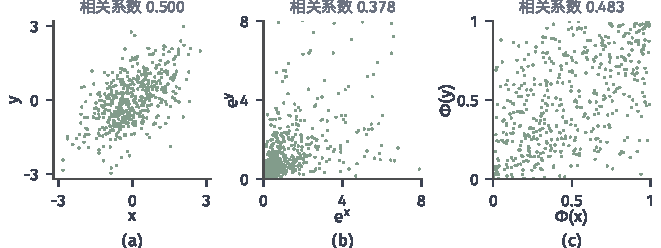
\includegraphics[width=112mm]{figures/07-probability/04-distribution-analysis/matplotlib/dep-mi-coordinates/figure.pdf}
  \caption{同一组标准二元高斯样本（$\rho=0.5$，$500$个，种子$719$）在三种坐标下。(a)原坐标；(b)$(\mathrm{e}^{x},\mathrm{e}^{y})$，有$15$个点超出画框；(c)$(\Phi(x),\Phi(y))$，即高斯Copula。图上方是各自的相关系数$\rho$、$(\mathrm{e}^{\rho}-1)/(\mathrm{e}-1)$与$(6/\pi)\arcsin(\rho/2)$；三者的互信息都是$-\frac12\ln0.75\approx0.144$。}
  \label{fig:dep-mi-coordinates}
\end{BookInlineFigure}

\paragraph{不可逆的处理}
若$f$不是一一的，式~\eqref{eq:dep-mi-processing}一般是严格不等式。在三点抛物线中只保留$X$是否为正，令$B=\mathbf{1}_{\{X>0\}}$。$B=1$时$X=1$，$Y=1$确定；$B=0$（概率$2/3$）时$X$等可能为$-1$或$0$，$Y$等可能为$1$或$0$，剩下$\ln2$的不确定性。于是
\[
  H(Y\mid B)=\tfrac23\ln2,\qquad I(B;Y)=H(Y)-H(Y\mid B)=\ln3-\tfrac43\ln2\approx0.174 .
\]
从$0.637$降到$0.174$：把$-1$和$0$合并以后，原来能区分的情形不再能区分。如果只合并$X$的$-1$与$1$，即改用$\lvert X\rvert$，那么$Y=\lvert X\rvert$仍由它确定，互信息不变。是否损失信息，看被合并的取值对另一个变量是否“有区别”。

\subsection{确定关系与无穷信息}
\label{sec:dep-mi-infinite}

三点抛物线的互信息是有限的$0.637$，那么连续抛物线$X\sim\operatorname{Unif}(-1,1)$，$Y=X^{2}$呢？$Y$同样由$X$确定，但它有不可数多个取值，“观测$X$后消除的不确定性”没有上限。

先看直观图景。联合分布的全部质量都在抛物线$y=x^{2}$上，这条曲线在平面上面积为零；边缘乘积则把质量摊在整个矩形$[-1,1]\times[0,1]$上，密度是$\frac12\cdot\frac{1}{2\sqrt{y}}$。在曲线周围取一条宽为$2\varepsilon$的带子$\{\lvert y-x^{2}\rvert\leq\varepsilon\}$。联合分布给它概率$1$，边缘乘积给它的概率记为$q_\varepsilon$，它随$\varepsilon\to0$趋于零。只记录“是否落在带子里”这个二值标签，由数据处理不等式，
\[
  I(X;Y)\geq D_{\mathrm{KL}}\bigl(\operatorname{Bern}(1)\,\Vert\,\operatorname{Bern}(q_\varepsilon)\bigr)=\ln\frac{1}{q_\varepsilon}.
\]
数值计算给出$q_{0.05}\approx0.134$，$q_{0.01}\approx0.035$，相应的下界约为$2.01$与$3.35$。带子越窄，下界越大，图~\ref{fig:dep-graph-band}画出了这一过程。

\begin{BookInlineFigure}
  \centering
  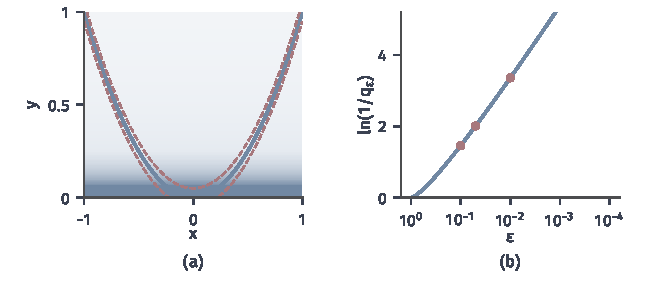
\includegraphics[width=110mm]{figures/07-probability/04-distribution-analysis/matplotlib/dep-graph-band/figure.pdf}
  \caption{质量在曲线上与质量摊开。(a)连续抛物线的边缘乘积密度$1/(4\sqrt{y})$（白到蓝，大于$1$的部分截断显示）；蓝线是联合分布的全部质量所在的曲线$y=x^{2}$，红色虚线围出带子$\lvert y-x^{2}\rvert\leq0.05$。(b)带子在边缘乘积下的概率$q_\varepsilon$给出的下界$\ln(1/q_\varepsilon)$，横轴向右$\varepsilon$减小；红点为$\varepsilon=0.1,0.05,0.01$，对应$1.46$、$2.01$、$3.35$。}
  \label{fig:dep-graph-band}
\end{BookInlineFigure}

下面的定理把“曲线面积为零”换成边缘乘积给图像零概率，给出一般结论。这里要求取值空间是标准Borel空间（第~\ref{chap:conditional-distributions}章引入，欧氏空间及其Borel子集都是），它保证了函数图像可测。

\begin{theorem}[确定关系的互信息]
\label{thm:dep-mi-infinite}
设$\mathcal{X},\mathcal{Y}$是标准Borel空间，$f:\mathcal{X}\to\mathcal{Y}$可测，$Y=f(X)$。若$Y$的分布无原子，即$\mathbb{P}(Y=y)=0$对每个$y\in\mathcal{Y}$成立，则
\begin{equation}
  I\bigl(X;f(X)\bigr)=+\infty .
  \label{eq:dep-mi-infinite}
\end{equation}
\end{theorem}

\begin{proof}
考虑$f$的图像$G=\{(x,y):y=f(x)\}$。标准Borel空间的对角线$\Delta=\{(y,y)\}$是$\mathcal{Y}\times\mathcal{Y}$中的可测集，而$G$是$\Delta$在可测映射$(x,y)\mapsto(f(x),y)$下的原像，所以$G$可测。

联合分布把全部质量放在$G$上：
\[
  P_{(X,Y)}(G)=\mathbb{P}\bigl(f(X)=Y\bigr)=1 .
\]
再算边缘乘积给$G$的概率。由乘积测度的截面公式（Tonelli定理），先固定$x$，截面$\{y:(x,y)\in G\}$只有一个点$f(x)$，于是
\[
  (P_X\otimes P_Y)(G)=\int_{\mathcal{X}}P_Y\bigl(\{f(x)\}\bigr)\,P_X(\mathrm{d}x)=0 ,
\]
最后一步用了$P_Y$无原子。一个集合在$P_X\otimes P_Y$下概率为零、在$P_{(X,Y)}$下概率为一，所以$P_{(X,Y)}$不绝对连续于$P_X\otimes P_Y$，按约定式~\eqref{eq:dep-mi}中的KL散度为$+\infty$。
\end{proof}

定理中两个条件各有作用。无原子保证了边缘乘积给图像零概率；若$Y$有原子，例如三点抛物线，图像的乘积概率为正，互信息有限。标准Borel保证图像可测，从而“质量全在图像上”有意义。函数$f$本身不需要连续或单调：$f(x)=x^{2}$不是一一的，结论照样成立。

\paragraph{有限与无穷的分界}
离散情形的对照是：若$Y=f(X)$只取有限多个值，那么给定$X$后$Y$没有不确定性，
\[
  I\bigl(X;f(X)\bigr)=H\bigl(f(X)\bigr)\leq\ln\lvert f(\mathcal{X})\rvert ,
\]
其中$\lvert f(\mathcal{X})\rvert$是取值个数。三点抛物线$H(Y)=0.637<\ln2$就是这种情形。可数无穷多个取值时，$H(f(X))$可以已经是无穷大；不可数且无原子时，定理~\ref{thm:dep-mi-infinite}说它一定是无穷大。所以互信息没有一个对所有分布都成立的有限上界，它的数值本身不能直接归一化到$[0,1]$。

加一点噪声，互信息又变成有限的。令$Y=X^{2}+\sigma Z$，$Z\sim\mathcal{N}(0,1)$与$X$独立。给定$X=x$时$Y\sim\mathcal{N}(x^{2},\sigma^{2})$，条件微分熵是$\frac12\ln(2\pi\mathrm{e}\sigma^{2})$，所以
\[
  I(X;Y)=h(Y)-\tfrac12\ln(2\pi\mathrm{e}\sigma^{2}),
\]
其中$h(Y)$对$Y$的密度（$X^{2}$的分布与$\mathcal{N}(0,\sigma^{2})$的卷积）数值积分得到。$\sigma=0.2$时约为$0.555$，$\sigma=0.1$时约为$1.03$。$\sigma\to0$时$h(Y)$趋于$X^{2}$的微分熵，而噪声项$-\frac12\ln(2\pi\mathrm{e}\sigma^{2})$像$\ln(1/\sigma)$那样增长，互信息随之发散。高斯情形的$-\frac12\ln(1-\rho^{2})$在$\lvert\rho\rvert\to1$时同样发散。图~\ref{fig:dep-mi-noise}把两种发散画在一起。

\begin{BookInlineFigure}
  \centering
  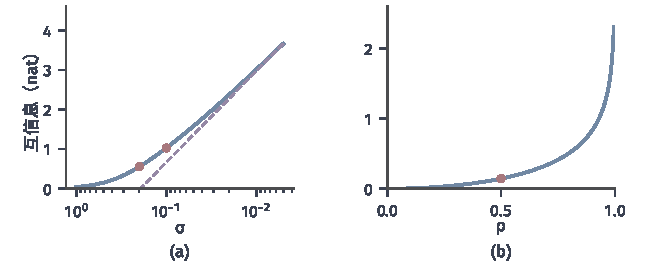
\includegraphics[width=110mm]{figures/07-probability/04-distribution-analysis/matplotlib/dep-mi-noise/figure.pdf}
  \caption{互信息向无穷大发散。(a)$I(X;X^{2}+\sigma Z)$随$\sigma$减小（横轴向右）而增大，蓝线由$h(Y)-\frac12\ln(2\pi\mathrm{e}\sigma^{2})$数值积分得到；紫色虚线是斜率与$\ln(1/\sigma)$相同的参考线；红点为$\sigma=0.2,0.1$，数值约$0.555$、$1.03$。(b)标准二元高斯的$I=-\frac12\ln(1-\rho^{2})$，红点为$\rho=0.5$处的$0.144$。}
  \label{fig:dep-mi-noise}
\end{BookInlineFigure}

\paragraph{下界不是数值}
真实互信息可以无穷大，计算上常用的却是有限的下界。第~\ref{chap:information-measures}章的InfoNCE下界在$N$个候选时不超过$\ln N$：对连续抛物线，$N=16$时它至多给出$\ln16\approx2.77$，而真实值是$+\infty$。下界给出“至少有这么多信息”，不能读成“信息就这么多”；两个分布的下界大小次序，也不一定是它们真实互信息的次序。


\section{距离协方差}
\label{sec:dep-distance-covariance}

互信息不看取值之间的距离，也没有有限上界。对欧氏空间中的随机向量，我们想要另一种度量：它的零值仍然刻画独立，数值又能用成对距离直接计算，并且有界。出发点是第~\ref{chap:weak-convergence-of-distributions}章的特征函数。设$\bm{X}$取值于$\mathbb{R}^{p}$，$\bm{Y}$取值于$\mathbb{R}^{q}$，联合特征函数为
\[
  \phi_{\bm{X},\bm{Y}}(\bm{t},\bm{s})=\mathbb{E}\bigl[\mathrm{e}^{\mathrm{i}\langle\bm{t},\bm{X}\rangle+\mathrm{i}\langle\bm{s},\bm{Y}\rangle}\bigr],\qquad \bm{t}\in\mathbb{R}^{p},\ \bm{s}\in\mathbb{R}^{q}.
\]
边缘乘积$P_{\bm{X}}\otimes P_{\bm{Y}}$的特征函数是$\phi_{\bm{X}}(\bm{t})\phi_{\bm{Y}}(\bm{s})$：在乘积空间上取独立的$\tilde{\bm{X}}\sim P_{\bm{X}}$、$\tilde{\bm{Y}}\sim P_{\bm{Y}}$，期望分解成乘积。特征函数确定分布，所以独立等价于两个特征函数处处相等。依赖的大小就用它们之差
\[
  \Delta(\bm{t},\bm{s})=\phi_{\bm{X},\bm{Y}}(\bm{t},\bm{s})-\phi_{\bm{X}}(\bm{t})\,\phi_{\bm{Y}}(\bm{s})
\]
在所有频率上的加权平方积分来量。关键在于选什么权重。

\subsection{定义与独立性}
\label{sec:dep-dcov-definition}

权重要满足三点：处处为正，才不会漏掉某个频段的差别；积分有限；最好还能把积分算回原来的取值空间。下面这个积分恒等式说明，幂次权重$\lVert\bm{t}\rVert_2^{-(d+1)}$把“频率空间里的$1-\cos$”变成“取值空间里的距离”。

\begin{lemma}[余弦积分与距离]
\label{lem:dep-cos-integral}
对$d\geq1$，记
\begin{equation}
  c_d=\int_{\mathbb{R}^{d}}\frac{1-\cos t_1}{\lVert\bm{t}\rVert_2^{d+1}}\,\mathrm{d}\bm{t},
  \label{eq:dep-cd}
\end{equation}
其中$t_1$是$\bm{t}$的第一个坐标。则$0<c_d<\infty$，$c_1=\pi$，并且对每个$\bm{x}\in\mathbb{R}^{d}$，
\begin{equation}
  \int_{\mathbb{R}^{d}}\frac{1-\cos\langle\bm{t},\bm{x}\rangle}{\lVert\bm{t}\rVert_2^{d+1}}\,\mathrm{d}\bm{t}=c_d\,\lVert\bm{x}\rVert_2 .
  \label{eq:dep-cos-integral}
\end{equation}
\end{lemma}

\begin{proof}
先证式~\eqref{eq:dep-cd}有限。在单位球内，
\[
  1-\cos t_1\leq\tfrac12t_1^{2}\leq\tfrac12\lVert\bm{t}\rVert_2^{2},
\]
被积函数不超过$\frac12\lVert\bm{t}\rVert_2^{1-d}$。用极坐标，$\mathbb{R}^{d}$中半径$r$的球面面积与$r^{d-1}$成正比，
\[
  \int_{\lVert\bm{t}\rVert_2\leq1}\lVert\bm{t}\rVert_2^{1-d}\,\mathrm{d}\bm{t}\ \propto\ \int_0^1r^{1-d}\,r^{d-1}\,\mathrm{d}r=1 .
\]
在单位球外，由$1-\cos t_1\leq2$，被积函数不超过$2\lVert\bm{t}\rVert_2^{-d-1}$，对应的径向积分为$\int_1^\infty r^{-2}\,\mathrm{d}r=1$。两部分都有限。被积函数非负，且在$t_1\notin2\pi\mathbb{Z}$处为正，所以$c_d>0$。

再证式~\eqref{eq:dep-cos-integral}。$\bm{x}=\bm{0}$时两边都是零。$\bm{x}\neq\bm{0}$时，取正交矩阵$\bm{R}$使$\bm{R}\bm{x}=\lVert\bm{x}\rVert_2\bm{e}_1$，作代换$\bm{u}=\bm{R}\bm{t}$。正交变换保持体积与范数，并且
\[
  \langle\bm{t},\bm{x}\rangle=\langle\bm{R}\bm{t},\bm{R}\bm{x}\rangle=\lVert\bm{x}\rVert_2u_1 ,
\]
所以左边变为
\[
  \int_{\mathbb{R}^{d}}\frac{1-\cos(\lVert\bm{x}\rVert_2u_1)}{\lVert\bm{u}\rVert_2^{d+1}}\,\mathrm{d}\bm{u}.
\]
再令$\bm{v}=\lVert\bm{x}\rVert_2\bm{u}$，体积元与分母分别变为
\[
  \mathrm{d}\bm{u}=\lVert\bm{x}\rVert_2^{-d}\,\mathrm{d}\bm{v},\qquad \lVert\bm{u}\rVert_2^{d+1}=\lVert\bm{x}\rVert_2^{-d-1}\lVert\bm{v}\rVert_2^{d+1},
\]
积分变为
\[
  \lVert\bm{x}\rVert_2^{d+1}\cdot\lVert\bm{x}\rVert_2^{-d}\int_{\mathbb{R}^{d}}\frac{1-\cos v_1}{\lVert\bm{v}\rVert_2^{d+1}}\,\mathrm{d}\bm{v}=c_d\,\lVert\bm{x}\rVert_2 .
\]

最后求$c_1$。三角形密度$f(x)=(1-\lvert x\rvert)^{+}$的特征函数是
\[
  \phi(t)=2\int_0^1(1-x)\cos(tx)\,\mathrm{d}x=\frac{2(1-\cos t)}{t^{2}},
\]
最后一步用分部积分：
\[
  \int_0^1(1-x)\cos(tx)\,\mathrm{d}x=\Bigl[(1-x)\frac{\sin tx}{t}\Bigr]_0^1+\int_0^1\frac{\sin tx}{t}\,\mathrm{d}x=\frac{1-\cos t}{t^{2}}.
\]$\phi$非负可积，由第~\ref{chap:weak-convergence-of-distributions}章的反演公式在$x=0$处，
\[
  1=f(0)=\frac{1}{2\pi}\int_{-\infty}^{\infty}\phi(t)\,\mathrm{d}t=\frac1\pi\int_{-\infty}^{\infty}\frac{1-\cos t}{t^{2}}\,\mathrm{d}t ,
\]
所以$c_1=\pi$。
\end{proof}

一般维数的常数是$c_d=\pi^{(d+1)/2}/\Gamma\bigl((d+1)/2\bigr)$，后面只用到它有限且为正，不需要具体数值。图~\ref{fig:dep-cos-kernel}画出$d=1$的被积函数：$x=2$的曲线在原点附近高出四倍、宽度减半，总面积恰好加倍。

\begin{BookInlineFigure}
  \centering
  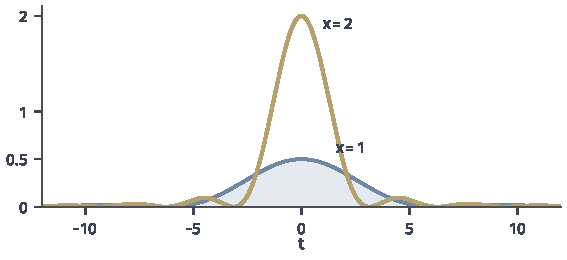
\includegraphics[width=96mm]{figures/07-probability/04-distribution-analysis/matplotlib/dep-cos-kernel/figure.pdf}
  \caption{引理~\ref{lem:dep-cos-integral}在$d=1$时的被积函数$(1-\cos tx)/t^{2}$。蓝线与浅蓝面积对应$x=1$，黄线对应$x=2$；两者在实轴上的积分分别为$\pi$与$2\pi$，与$\lvert x\rvert$成正比（数值积分在$[-4000,4000]$上得$3.1401$与$6.2787$，截去的尾部不超过$2/4000$与$4/4000$）。}
  \label{fig:dep-cos-kernel}
\end{BookInlineFigure}

现在用这个权重定义距离协方差。

\begin{definition}[距离协方差]
\label{def:dep-dcov}
设$\bm{X}\in\mathbb{R}^{p}$、$\bm{Y}\in\mathbb{R}^{q}$满足$\mathbb{E}\lVert\bm{X}\rVert_2<\infty$、$\mathbb{E}\lVert\bm{Y}\rVert_2<\infty$。$\bm{X}$与$\bm{Y}$的\term{距离协方差}（distance covariance）的平方定义为
\begin{equation}
  \operatorname{dCov}^{2}(\bm{X},\bm{Y})=\frac{1}{c_pc_q}\int_{\mathbb{R}^{p+q}}\frac{\lvert\Delta(\bm{t},\bm{s})\rvert^{2}}{\lVert\bm{t}\rVert_2^{p+1}\lVert\bm{s}\rVert_2^{q+1}}\,\mathrm{d}\bm{t}\,\mathrm{d}\bm{s},
  \label{eq:dep-dcov-def}
\end{equation}
其中$\Delta$是联合特征函数与边缘特征函数乘积之差。它的非负平方根记为$\operatorname{dCov}(\bm{X},\bm{Y})$。
\end{definition}

被积函数非负，积分总有意义，下面的定理说明一阶矩条件保证它有限，并且零值恰好刻画独立。

\begin{theorem}[距离协方差的有限性与零值]
\label{thm:dep-dcov-independence}
在定义~\ref{def:dep-dcov}的条件下，设$\bm{X}'$是$\bm{X}$的独立复制，$\bm{Y}'$是$\bm{Y}$的独立复制。则
\begin{equation}
  0\leq\operatorname{dCov}^{2}(\bm{X},\bm{Y})\leq\mathbb{E}\lVert\bm{X}-\bm{X}'\rVert_2\ \mathbb{E}\lVert\bm{Y}-\bm{Y}'\rVert_2<\infty ,
  \label{eq:dep-dcov-bound}
\end{equation}
并且$\operatorname{dCov}^{2}(\bm{X},\bm{Y})=0$当且仅当$\bm{X}$与$\bm{Y}$独立。
\end{theorem}

\begin{proof}
\emph{有限性。}把$\Delta$写成两个中心化复指数乘积的期望。展开右边并逐项取期望，
\[
  \mathbb{E}\Bigl[\bigl(\mathrm{e}^{\mathrm{i}\langle\bm{t},\bm{X}\rangle}-\phi_{\bm{X}}(\bm{t})\bigr)\bigl(\mathrm{e}^{\mathrm{i}\langle\bm{s},\bm{Y}\rangle}-\phi_{\bm{Y}}(\bm{s})\bigr)\Bigr]=\phi_{\bm{X},\bm{Y}}-\phi_{\bm{X}}\phi_{\bm{Y}}-\phi_{\bm{Y}}\phi_{\bm{X}}+\phi_{\bm{X}}\phi_{\bm{Y}},
\]
右边正是$\Delta(\bm{t},\bm{s})$。对复值随机变量用Cauchy--Schwarz不等式
\[
  \lvert\mathbb{E}[UV]\rvert^{2}\leq\mathbb{E}\lvert U\rvert^{2}\,\mathbb{E}\lvert V\rvert^{2},
\]
并注意
\[
  \mathbb{E}\bigl\lvert\mathrm{e}^{\mathrm{i}\langle\bm{t},\bm{X}\rangle}-\phi_{\bm{X}}(\bm{t})\bigr\rvert^{2}=1-\lvert\phi_{\bm{X}}(\bm{t})\rvert^{2},
\]
得到
\[
  \lvert\Delta(\bm{t},\bm{s})\rvert^{2}\leq\bigl(1-\lvert\phi_{\bm{X}}(\bm{t})\rvert^{2}\bigr)\bigl(1-\lvert\phi_{\bm{Y}}(\bm{s})\rvert^{2}\bigr).
\]
右边分离了$\bm{t}$与$\bm{s}$。用独立复制$\bm{X}'$把共轭$\overline{\phi_{\bm{X}}(\bm{t})}$写成$\mathbb{E}\,\mathrm{e}^{-\mathrm{i}\langle\bm{t},\bm{X}'\rangle}$，再取实部，
\[
  1-\lvert\phi_{\bm{X}}(\bm{t})\rvert^{2}=1-\mathbb{E}\,\mathrm{e}^{\mathrm{i}\langle\bm{t},\bm{X}-\bm{X}'\rangle}=\mathbb{E}\bigl[1-\cos\langle\bm{t},\bm{X}-\bm{X}'\rangle\bigr].
\]被积函数非负，由Tonelli定理交换积分与期望，再用引理~\ref{lem:dep-cos-integral}，
\[
  \int_{\mathbb{R}^{p}}\frac{1-\lvert\phi_{\bm{X}}(\bm{t})\rvert^{2}}{\lVert\bm{t}\rVert_2^{p+1}}\,\mathrm{d}\bm{t}=c_p\,\mathbb{E}\lVert\bm{X}-\bm{X}'\rVert_2 .
\]
$\bm{Y}$一侧同理。两式相乘再除以$c_pc_q$，就是式~\eqref{eq:dep-dcov-bound}。由三角不等式，$\mathbb{E}\lVert\bm{X}-\bm{X}'\rVert_2$不超过$2\,\mathbb{E}\lVert\bm{X}\rVert_2<\infty$。

\emph{零值。}若$\bm{X},\bm{Y}$独立，则$\mathrm{e}^{\mathrm{i}\langle\bm{t},\bm{X}\rangle}$与$\mathrm{e}^{\mathrm{i}\langle\bm{s},\bm{Y}\rangle}$独立，期望分解，$\Delta\equiv0$，积分为零。反之，若积分为零，权重处处为正（除去测度为零的坐标面），所以$\lvert\Delta\rvert^{2}=0$几乎处处成立。特征函数连续，$\lvert\Delta\rvert^{2}$连续；一个连续的非负函数若在某点为正，就在该点的一个邻域内为正，邻域测度为正，与几乎处处为零矛盾。所以$\Delta\equiv0$，即$(\bm{X},\bm{Y})$与$(\tilde{\bm{X}},\tilde{\bm{Y}})$的特征函数相同。由第~\ref{chap:weak-convergence-of-distributions}章的唯一性定理，$P_{(\bm{X},\bm{Y})}=P_{\bm{X}}\otimes P_{\bm{Y}}$。
\end{proof}

\paragraph{三点抛物线}
这个例子的特征函数可以直接写出。三个等可能的点是$(-1,1)$、$(0,0)$、$(1,1)$，所以
\[
  \begin{gathered}
  \phi_{X,Y}(t,s)=\tfrac13\bigl(1+2\cos t\,\mathrm{e}^{\mathrm{i}s}\bigr),\\
  \phi_X(t)=\tfrac13(1+2\cos t),\qquad \phi_Y(s)=\tfrac13(1+2\mathrm{e}^{\mathrm{i}s}).
  \end{gathered}
\]
相减并合并同类项，
\[
  \Delta(t,s)=\frac{3+6\cos t\,\mathrm{e}^{\mathrm{i}s}-(1+2\cos t)(1+2\mathrm{e}^{\mathrm{i}s})}{9}=\frac{2(1-\cos t)(1-\mathrm{e}^{\mathrm{i}s})}{9}.
\]
$1-\mathrm{e}^{\mathrm{i}s}$的模平方是$(1-\cos s)^{2}+\sin^{2}s=2(1-\cos s)$，所以
\[
  \lvert\Delta(t,s)\rvert^{2}=\frac{8}{81}(1-\cos t)^{2}(1-\cos s).
\]
它在$t=0$或$s=0$的坐标轴上为零：只看一个变量时，联合分布与边缘乘积没有差别。

代入式~\eqref{eq:dep-dcov-def}（$p=q=1$，$c_1=\pi$），积分分离成两个一维积分。$s$一侧由引理~\ref{lem:dep-cos-integral}是$\pi$。$t$一侧用$(1-\cos t)^{2}=2(1-\cos t)-\frac12(1-\cos2t)$，再分别套用引理，
\[
  \int_{-\infty}^{\infty}\frac{(1-\cos t)^{2}}{t^{2}}\,\mathrm{d}t=2\pi-\tfrac12\cdot2\pi=\pi .
\]
于是
\[
  \operatorname{dCov}^{2}(X,Y)=\frac{1}{\pi^{2}}\cdot\frac{8}{81}\cdot\pi\cdot\pi=\frac{8}{81}\approx0.0988 .
\]
图~\ref{fig:dep-cf-gap}画出了$\lvert\Delta\rvert^{2}$与加权后的被积函数。

\begin{BookInlineFigure}
  \centering
  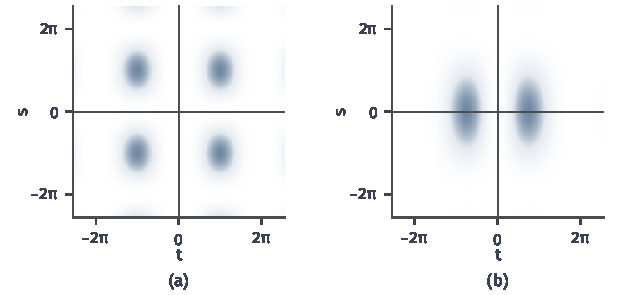
\includegraphics[width=108mm]{figures/07-probability/04-distribution-analysis/matplotlib/dep-cf-gap/figure.pdf}
  \caption{三点抛物线的特征函数之差。(a)$\lvert\Delta(t,s)\rvert^{2}=\frac{8}{81}(1-\cos t)^{2}(1-\cos s)$，白到蓝表示由小到大，在两条坐标轴上为零；(b)加权被积函数$\lvert\Delta\rvert^{2}/(\pi^{2}t^{2}s^{2})$，权重压低了高频，质量集中在$\lvert t\rvert\approx2$、$s$接近零的两块。(b)在全平面上的积分为$8/81$。}
  \label{fig:dep-cf-gap}
\end{BookInlineFigure}

\paragraph{权重不能随意替换}
零值判据的证明只用到权重处处为正与特征函数的唯一性；如果权重只在有界区域上为正，可能漏掉在那个区域外才出现的差别，因为两个不同的分布，其特征函数可以在一个区间上相同。权重的幂次也不能随意改动。若把$\lVert\bm{t}\rVert_2^{-(d+1)}$换成$\lVert\bm{t}\rVert_2^{-(d+\alpha)}$，引理的同样论证给出
\[
  \int_{\mathbb{R}^{d}}\frac{1-\cos\langle\bm{t},\bm{x}\rangle}{\lVert\bm{t}\rVert_2^{d+\alpha}}\,\mathrm{d}\bm{t}=c_{d,\alpha}\lVert\bm{x}\rVert_2^{\alpha},
\]
有限性要求原点附近$\lVert\bm{t}\rVert_2^{2-d-\alpha}$可积，即$\alpha<2$，无穷远处$\lVert\bm{t}\rVert_2^{-d-\alpha}$可积，即$\alpha>0$。所以$0<\alpha<2$时得到以$\lVert\bm{x}-\bm{x}'\rVert_2^{\alpha}$代替距离的一族度量，需要$\alpha$阶矩；$\alpha=2$时积分发散，下一小节会看到，强行把距离换成平方距离，零值判据就失效了。

\subsection{成对距离的表示}
\label{sec:dep-dcov-pairwise}

式~\eqref{eq:dep-dcov-def}是频率空间里的积分，实际计算时我们更希望回到取值空间。引理~\ref{lem:dep-cos-integral}已经把$1-\cos$换成距离，剩下的工作是把$\lvert\Delta\rvert^{2}$展开成若干个$1-\cos$的期望。为此引入$(\bm{X},\bm{Y})$的两个独立复制$(\bm{X}',\bm{Y}')$与$(\bm{X}'',\bm{Y}'')$，三组相互独立、同分布。

\begin{theorem}[距离协方差的成对距离表示]
\label{thm:dep-dcov-pairwise}
设$\mathbb{E}\lVert\bm{X}\rVert_2^{2}<\infty$，$\mathbb{E}\lVert\bm{Y}\rVert_2^{2}<\infty$。记$a=\lVert\bm{X}-\bm{X}'\rVert_2$，$b=\lVert\bm{Y}-\bm{Y}'\rVert_2$，$b''=\lVert\bm{Y}-\bm{Y}''\rVert_2$。则
\begin{equation}
  \operatorname{dCov}^{2}(\bm{X},\bm{Y})=\mathbb{E}[ab]+\mathbb{E}[a]\,\mathbb{E}[b]-2\,\mathbb{E}[ab''] .
  \label{eq:dep-dcov-pairwise}
\end{equation}
\end{theorem}

\begin{proof}
固定$(\bm{t},\bm{s})$，记三个随机相位
\[
  \theta=\langle\bm{t},\bm{X}-\bm{X}'\rangle,\qquad \eta=\langle\bm{s},\bm{Y}-\bm{Y}'\rangle,\qquad \eta''=\langle\bm{s},\bm{Y}-\bm{Y}''\rangle .
\]
用独立复制把$\lvert\Delta\rvert^{2}=\Delta\overline{\Delta}$的四项写成期望：
\[
  \begin{aligned}
    \phi_{\bm{X},\bm{Y}}\overline{\phi_{\bm{X},\bm{Y}}}&=\mathbb{E}\,\mathrm{e}^{\mathrm{i}(\theta+\eta)},\qquad
    \lvert\phi_{\bm{X}}\phi_{\bm{Y}}\rvert^{2}=\mathbb{E}\,\mathrm{e}^{\mathrm{i}\theta}\ \mathbb{E}\,\mathrm{e}^{\mathrm{i}\eta},\\
    \phi_{\bm{X},\bm{Y}}\overline{\phi_{\bm{X}}\phi_{\bm{Y}}}&=\mathbb{E}\,\mathrm{e}^{\mathrm{i}(\theta+\eta'')} .
  \end{aligned}
\]
第三项中$\overline{\phi_{\bm{X}}(\bm{t})}$用第二组复制写成期望，$\overline{\phi_{\bm{Y}}(\bm{s})}$用第三组复制。第四项是第三项的共轭。$\theta$与$-\theta$同分布，所以$\mathbb{E}\sin\theta=0$，同理$\mathbb{E}\sin\eta=0$。取实部，
\[
  \lvert\Delta\rvert^{2}=\mathbb{E}\cos\theta\cos\eta+\mathbb{E}\cos\theta\,\mathbb{E}\cos\eta-2\,\mathbb{E}\cos\theta\cos\eta''+S(\bm{t},\bm{s}),
\]
其中正弦部分为
\[
  S(\bm{t},\bm{s})=-\mathbb{E}\sin\theta\sin\eta+2\,\mathbb{E}\sin\theta\sin\eta'' .
\]

把$\cos\theta\cos\eta$写成$1-(1-\cos\theta)-(1-\cos\eta)+(1-\cos\theta)(1-\cos\eta)$，对另外两项同样展开。$\eta$与$\eta''$同分布，三项中常数与单个$1-\cos$的部分按系数$1+1-2=0$全部抵消。记$G(\bm{t},\bm{s})$为剩下的部分，
\[
  \begin{aligned}
  G={}&\mathbb{E}\bigl[(1-\cos\theta)(1-\cos\eta)\bigr]+\mathbb{E}[1-\cos\theta]\,\mathbb{E}[1-\cos\eta]\\
  &-2\,\mathbb{E}\bigl[(1-\cos\theta)(1-\cos\eta'')\bigr],
  \end{aligned}
\]
于是$\lvert\Delta\rvert^{2}=G+S$。

$S$关于$\bm{t}$是奇函数（$\bm{t}\to-\bm{t}$时$\sin\theta$变号），$G$是偶函数。权重关于$\bm{t}$对称，用代换$\bm{t}\to-\bm{t}$把式~\eqref{eq:dep-dcov-def}写成$\frac12(\lvert\Delta(\bm{t},\bm{s})\rvert^{2}+\lvert\Delta(-\bm{t},\bm{s})\rvert^{2})$的积分，这个平均正好是$G$。这一步只涉及非负函数的积分，不需要$S$可积。所以
\[
  \operatorname{dCov}^{2}(\bm{X},\bm{Y})=\frac{1}{c_pc_q}\int_{\mathbb{R}^{p+q}}\frac{G(\bm{t},\bm{s})}{\lVert\bm{t}\rVert_2^{p+1}\lVert\bm{s}\rVert_2^{q+1}}\,\mathrm{d}\bm{t}\,\mathrm{d}\bm{s}.
\]

$G$的三项各自是非负函数的期望。对第一项用Tonelli定理交换期望与积分，两次运用引理~\ref{lem:dep-cos-integral}，
\[
  \frac{1}{c_pc_q}\int\!\!\int\frac{\mathbb{E}[(1-\cos\theta)(1-\cos\eta)]}{\lVert\bm{t}\rVert_2^{p+1}\lVert\bm{s}\rVert_2^{q+1}}\,\mathrm{d}\bm{t}\,\mathrm{d}\bm{s}=\mathbb{E}[ab].
\]
第二、三项同理分别得到$\mathbb{E}[a]\mathbb{E}[b]$与$\mathbb{E}[ab'']$。由Cauchy--Schwarz不等式，$\mathbb{E}[ab]$不超过$(\mathbb{E}a^{2}\,\mathbb{E}b^{2})^{1/2}$，而由三角不等式$\mathbb{E}a^{2}$不超过$4\,\mathbb{E}\lVert\bm{X}\rVert_2^{2}$，是有限的，三项都有限，可以按线性逐项积分，得到式~\eqref{eq:dep-dcov-pairwise}。
\end{proof}

\paragraph{为什么需要二阶矩}
定义~\ref{def:dep-dcov}只需要一阶矩，式~\eqref{eq:dep-dcov-pairwise}却要求三项分别有限。只有一阶矩时，左边仍有限，右边可能是$\infty-\infty$。取$Y=X$，$X$服从第~\ref{chap:laws-of-large-numbers}章用过的$\alpha=1.5$的Pareto分布，$\mathbb{E}\lvert X\rvert<\infty$而$\mathbb{E}X^{2}=\infty$。这时$\mathbb{E}[ab]$就是$\mathbb{E}\lvert X-X'\rvert^{2}=\infty$，$\mathbb{E}[ab'']$也是无穷大，式~\eqref{eq:dep-dcov-pairwise}右边没有意义；而由式~\eqref{eq:dep-dcov-bound}，左边不超过$(\mathbb{E}\lvert X-X'\rvert)^{2}$，是有限的。二阶矩是让逐项展开合法的充分条件，不是距离协方差存在的条件。

\paragraph{双重中心化}
式~\eqref{eq:dep-dcov-pairwise}还可以写成一个“协方差”的样子。记$m(\bm{x})=\mathbb{E}\lVert\bm{x}-\bm{X}'\rVert_2$为点$\bm{x}$到$\bm{X}$的平均距离，$D=\mathbb{E}\lVert\bm{X}-\bm{X}'\rVert_2$。对成对距离作\term{双重中心化}（double centering），
\begin{equation}
  A(\bm{x},\bm{x}')=\lVert\bm{x}-\bm{x}'\rVert_2-m(\bm{x})-m(\bm{x}')+D ,
  \label{eq:dep-double-centering}
\end{equation}
即减去两端各自的平均距离，再加回总平均。对$\bm{Y}$同样定义$B(\bm{y},\bm{y}')$。则在定理~\ref{thm:dep-dcov-pairwise}的条件下
\begin{equation}
  \operatorname{dCov}^{2}(\bm{X},\bm{Y})=\mathbb{E}\bigl[A(\bm{X},\bm{X}')\,B(\bm{Y},\bm{Y}')\bigr].
  \label{eq:dep-dcov-centered}
\end{equation}

验证如下。记$n,D_Y$为$\bm{Y}$一侧与$m,D$对应的量。固定$\bm{y}$，对$\bm{Y}'$取期望，
\[
  \mathbb{E}\,B(\bm{y},\bm{Y}')=n(\bm{y})-n(\bm{y})-D_Y+D_Y=0 .
\]所以在$A$的四项中，只依赖$(\bm{X},\bm{Y})$一组的$m(\bm{X})$，与$B(\bm{Y},\bm{Y}')$相乘后先对$(\bm{X}',\bm{Y}')$取期望，得到零；$m(\bm{X}')$与常数$D$同理。只剩
\[
  \mathbb{E}\bigl[a\,B(\bm{Y},\bm{Y}')\bigr]=\mathbb{E}[ab]-\mathbb{E}\bigl[a\,n(\bm{Y})\bigr]-\mathbb{E}\bigl[a\,n(\bm{Y}')\bigr]+\mathbb{E}[a]\,D_Y .
\]
$n(\bm{Y})$是$b''$在给定$\bm{Y}$时的条件期望，所以$\mathbb{E}[a\,n(\bm{Y})]=\mathbb{E}[ab'']$；交换两组复制的角色，$\mathbb{E}[a\,n(\bm{Y}')]$也等于$\mathbb{E}[ab'']$。代回去就是式~\eqref{eq:dep-dcov-pairwise}的右边。

式~\eqref{eq:dep-dcov-centered}给出了一个直观的读法。$A(\bm{X},\bm{X}')>0$表示这一对$\bm{X}$比按各自位置预期的更远，$B>0$表示这一对$\bm{Y}$更远；距离协方差问的是“$\bm{X}$这对远时$\bm{Y}$这对是否也远”。中心化消去了只由一个边缘决定的部分：$m(\bm{x})$大只说明$\bm{x}$处在边缘分布的外围，与$\bm{Y}$无关。若$\bm{X},\bm{Y}$独立，则$(\bm{X},\bm{X}')$与$(\bm{Y},\bm{Y}')$独立，期望分解为$\mathbb{E}A\cdot\mathbb{E}B=0$。

\paragraph{平方距离只剩协方差}
现在可以看清为什么不能用平方距离。对实值变量把$\lvert x-x'\rvert$换成$(x-x')^{2}$，记$\mu=\mathbb{E}X$。$(x-x')^{2}$的平均是$m_2(x)=(x-\mu)^{2}+\operatorname{Var}(X)$，总平均是$2\operatorname{Var}(X)$，双重中心化后
\[
  (x-x')^{2}-m_2(x)-m_2(x')+2\operatorname{Var}(X)=-2(x-\mu)(x'-\mu).
\]
代入式~\eqref{eq:dep-dcov-centered}的形式，两组复制独立，
\[
  4\,\mathbb{E}\bigl[(X-\mu)(Y-\nu)(X'-\mu)(Y'-\nu)\bigr]=4\operatorname{Cov}(X,Y)^{2},
\]
其中$\nu=\mathbb{E}Y$。平方距离只保留了协方差，抛物线上为零；正是指数$1<2$使距离协方差看到了非线性的依赖。

\paragraph{三点抛物线的成对距离}
用式~\eqref{eq:dep-dcov-pairwise}重算三点抛物线。三个点的$x$坐标为$-1,0,1$，$y$坐标为$1,0,1$，成对距离矩阵为
\[
  \bm{A}=\begin{pmatrix}0&1&2\\1&0&1\\2&1&0\end{pmatrix},\qquad
  \bm{B}=\begin{pmatrix}0&1&0\\1&0&1\\0&1&0\end{pmatrix}.
\]
三点等可能，期望就是对$9$个元素求平均。第一项$\mathbb{E}[ab]$只在$\bm{B}$非零的四个位置有贡献，那里$\bm{A}$的元素都是$1$，
\[
  \mathbb{E}[ab]=\tfrac49,\qquad \mathbb{E}[a]=\tfrac89,\qquad \mathbb{E}[b]=\tfrac49 .
\]

第三项要先求每个点的平均距离：$\bm{A}$的行平均是$m=(1,\frac23,1)$，$\bm{B}$的行平均是$n=(\frac13,\frac23,\frac13)$。由$\mathbb{E}[ab'']=\mathbb{E}[m(X)\,n(Y)]$，
\[
  \mathbb{E}[ab'']=\tfrac13\Bigl(1\cdot\tfrac13+\tfrac23\cdot\tfrac23+1\cdot\tfrac13\Bigr)=\tfrac{10}{27}.
\]
代入式~\eqref{eq:dep-dcov-pairwise}，
\[
  \operatorname{dCov}^{2}(X,Y)=\frac49+\frac89\cdot\frac49-2\cdot\frac{10}{27}=\frac{36+32-60}{81}=\frac{8}{81},
\]
与特征函数积分的结果一致。

图~\ref{fig:dep-double-centering}给出双重中心化后的矩阵$\tilde{\bm{A}}$、$\tilde{\bm{B}}$：每行每列之和为零。按式~\eqref{eq:dep-dcov-centered}逐格相乘求和，
\[
  \frac19\sum_{i,j}\tilde{A}_{i,j}\tilde{B}_{i,j}=\frac19\cdot\frac{72}{81}=\frac{8}{81}.
\]

\begin{BookInlineFigure}
  \centering
  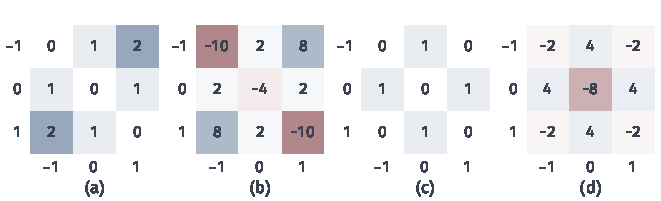
\includegraphics[width=112mm]{figures/07-probability/04-distribution-analysis/matplotlib/dep-double-centering/figure.pdf}
  \caption{三点抛物线的成对距离与双重中心化，行列按$x=-1,0,1$排列。(a)$\bm{A}=(\lvert x_i-x_j\rvert)$；(b)$\tilde{\bm{A}}$，格中数字乘以$1/9$；(c)$\bm{B}=(\lvert y_i-y_j\rvert)$；(d)$\tilde{\bm{B}}$，格中数字乘以$1/9$。(a)(c)白到蓝表示由小到大，(b)(d)红—白—蓝表示由负到正。中心化后每行每列之和为零。}
  \label{fig:dep-double-centering}
\end{BookInlineFigure}

$n$个样本点的经验分布也是这样一个等可能的有限分布，把式~\eqref{eq:dep-dcov-pairwise}用在经验分布上，就得到样本距离协方差。它作为总体量估计的性质，属于统计推断的问题。

\subsection{距离相关}
\label{sec:dep-dcor}

距离协方差有量纲：把$\bm{Y}$的单位从米换成厘米，$\operatorname{dCov}^{2}$乘以$100$。与由协方差得到相关系数一样，用各自的“距离方差”归一化。

\begin{definition}[距离相关]
\label{def:dep-dcor}
在定义~\ref{def:dep-dcov}的条件下，称$\bm{X}$与自身的距离协方差$\operatorname{dCov}^{2}(\bm{X},\bm{X})$为$\bm{X}$的\term{距离方差}（distance variance），记为$\operatorname{dVar}^{2}(\bm{X})$。$\bm{X}$与$\bm{Y}$的\term{距离相关}（distance correlation）定义为
\begin{equation}
  \operatorname{dCor}(\bm{X},\bm{Y})=
  \begin{cases}
    \dfrac{\operatorname{dCov}(\bm{X},\bm{Y})}{\sqrt{\operatorname{dVar}(\bm{X})\operatorname{dVar}(\bm{Y})}}, & \operatorname{dVar}(\bm{X})\operatorname{dVar}(\bm{Y})>0,\\
    0, & \operatorname{dVar}(\bm{X})\operatorname{dVar}(\bm{Y})=0 .
  \end{cases}
  \label{eq:dep-dcor}
\end{equation}
\end{definition}

第二行的约定只在常量情形起作用。由定理~\ref{thm:dep-dcov-independence}，$\operatorname{dVar}^{2}(\bm{X})=0$当且仅当$\bm{X}$与自身独立；这时对每个Borel集$C$，事件$\{\bm{X}\in C\}$与自身独立，它的概率$r$满足$r=r^{2}$，只能是$0$或$1$，每个坐标的分布函数只取$0,1$两个值，$\bm{X}$几乎必然是常数。常数与任何变量都独立，取距离相关为$0$与零值判据相容。

\begin{theorem}[距离相关的范围与不变性]
\label{thm:dep-dcor-properties}
在定义~\ref{def:dep-dcor}的条件下：
\begin{enumerate}
  \item $0\leq\operatorname{dCor}(\bm{X},\bm{Y})\leq1$，并且$\operatorname{dCor}(\bm{X},\bm{Y})=0$当且仅当$\bm{X}$与$\bm{Y}$独立；
  \item 对向量$\bm{a}_1\in\mathbb{R}^{p}$、$\bm{a}_2\in\mathbb{R}^{q}$，非零标量$b_1,b_2$与正交矩阵$\bm{C}_1,\bm{C}_2$，
  \begin{equation}
    \operatorname{dCov}^{2}(\bm{a}_1+b_1\bm{C}_1\bm{X},\ \bm{a}_2+b_2\bm{C}_2\bm{Y})=\lvert b_1b_2\rvert\operatorname{dCov}^{2}(\bm{X},\bm{Y}),
    \label{eq:dep-dcov-scaling}
  \end{equation}
  从而距离相关在这类变换下不变。
\end{enumerate}
\end{theorem}

\begin{proof}
零值部分由定理~\ref{thm:dep-dcov-independence}与常量约定直接得到。上界先在二阶矩有限时证明。由式~\eqref{eq:dep-dcov-centered}与Cauchy--Schwarz不等式，
\[
  \operatorname{dCov}^{2}(\bm{X},\bm{Y})\leq\bigl(\mathbb{E}A^{2}\bigr)^{1/2}\bigl(\mathbb{E}B^{2}\bigr)^{1/2}=\operatorname{dVar}(\bm{X})\operatorname{dVar}(\bm{Y}),
\]
最后一步对$\bm{Y}=\bm{X}$与$\bm{X}=\bm{Y}$再用一次式~\eqref{eq:dep-dcov-centered}。两边开方，除以$\operatorname{dVar}(\bm{X})\operatorname{dVar}(\bm{Y})$，得$\operatorname{dCor}\leq1$。

对第二部分，记$\bm{X}^{*}=\bm{a}_1+b_1\bm{C}_1\bm{X}$，它的特征函数为
\[
  \phi_{\bm{X}^{*}}(\bm{t})=\mathrm{e}^{\mathrm{i}\langle\bm{t},\bm{a}_1\rangle}\phi_{\bm{X}}\bigl(b_1\bm{C}_1^{\top}\bm{t}\bigr),
\]
联合特征函数同理。平移因子的模为$1$，所以变换后的差$\Delta^{*}$满足
\[
  \lvert\Delta^{*}(\bm{t},\bm{s})\rvert=\bigl\lvert\Delta\bigl(b_1\bm{C}_1^{\top}\bm{t},\,b_2\bm{C}_2^{\top}\bm{s}\bigr)\bigr\rvert .
\]
在式~\eqref{eq:dep-dcov-def}中作代换$\bm{u}=b_1\bm{C}_1^{\top}\bm{t}$。体积元变为$\lvert b_1\rvert^{-p}\mathrm{d}\bm{u}$，分母变为$\lvert b_1\rvert^{-p-1}\lVert\bm{u}\rVert_2^{p+1}$，积分多出因子$\lvert b_1\rvert$。$\bm{s}$一侧同样多出$\lvert b_2\rvert$，这就是式~\eqref{eq:dep-dcov-scaling}。对$\operatorname{dVar}^{2}$分别多出$b_1^{2}$与$b_2^{2}$，代入式~\eqref{eq:dep-dcor}相消。
\end{proof}

上界的证明用到了二阶矩。只有一阶矩时上界同样成立，需要先截断再验证各项的连续性，篇幅较长，可查阅\scite{math-szekely2007dependence}。

距离相关取到$1$的情形也已清楚：$\operatorname{dCor}(\bm{X},\bm{Y})=1$当且仅当$\bm{Y}=\bm{a}+b\bm{C}\bm{X}$几乎必然成立，其中$b\neq0$为标量、$\bm{C}$为正交矩阵，证明见同一文献。所以距离相关为$1$意味着两组坐标只差一个相似变换，比“$\bm{Y}$由$\bm{X}$确定”严格得多。

\paragraph{三点抛物线与高斯}
三点抛物线的距离方差由图~\ref{fig:dep-double-centering}的矩阵算出。中心化一侧即可，
\[
  \operatorname{dVar}^{2}(X)=\frac19\sum_{i,j}\tilde{A}_{i,j}A_{i,j}=\frac{40}{81},\qquad \operatorname{dVar}^{2}(Y)=\frac19\sum_{i,j}\tilde{B}_{i,j}B_{i,j}=\frac{16}{81}.
\]代入式~\eqref{eq:dep-dcor}，
\[
  \operatorname{dCor}^{2}(X,Y)=\frac{8/81}{\sqrt{(40/81)(16/81)}}=\frac{8}{\sqrt{640}}=\frac{1}{\sqrt{10}},
\]
所以$\operatorname{dCor}(X,Y)=10^{-1/4}\approx0.562$。$Y$由$X$确定，距离相关却远小于$1$，因为$Y=X^{2}$不是$X$的相似变换。

同一文献还算出了标准二元高斯的闭式结果：
\[
  \operatorname{dCor}^{2}=\frac{\rho\arcsin\rho+\sqrt{1-\rho^{2}}-\rho\arcsin(\rho/2)-\sqrt{4-\rho^{2}}+1}{1+\pi/3-\sqrt3}.
\]
$\rho=0.5$时约为$0.206$，即$\operatorname{dCor}\approx0.454$。图~\ref{fig:dep-dcor-gaussian}显示距离相关在高斯族内随$\lvert\rho\rvert$单调增，略低于$\lvert\rho\rvert$，两端与之重合。在高斯族内两者给出相同的次序，只是刻度不同。

\begin{BookInlineFigure}
  \centering
  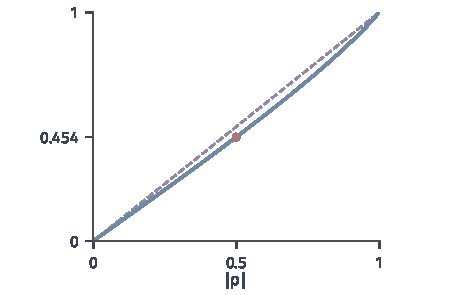
\includegraphics[width=80mm]{figures/07-probability/04-distribution-analysis/matplotlib/dep-dcor-gaussian/figure.pdf}
  \caption{标准二元高斯的距离相关随$\lvert\rho\rvert$的变化（蓝，闭式公式；脚本另用$60\times60$个Gauss--Hermite节点数值核对，相对误差在$0.3\%$以内）。紫色虚线是参考线$\lvert\rho\rvert$。红点为$\rho=0.5$处的$0.454$。}
  \label{fig:dep-dcor-gaussian}
\end{BookInlineFigure}

\paragraph{哪些变换保持距离相关}
定理~\ref{thm:dep-dcor-properties}允许的变换是平移、旋转（含反射）与同一个非零标量的整体缩放，它们保持距离之间的比例。其他变换一般会改变距离相关。把三点抛物线中$X$的取值$-1,0,1$改成$-1,0,5$，互信息不变，距离相关从$0.562$变为$0.530$。对高斯向量作坐标变换$(\mathrm{e}^{X},\mathrm{e}^{Y})$，距离相关从$0.454$变为约$0.42$；用$\Phi$变到Copula坐标，约为$0.45$；把$Y$整体乘以$10$则不变。图~\ref{fig:dep-transform-bars}把相关系数、距离相关与互信息放在一起比较：互信息在四种变换下都不动，距离相关只在相似变换下不动。若对$\bm{X}$的不同坐标用不同的比例缩放，例如$\operatorname{diag}(1,10)$，距离的比例被打乱，距离相关一般也会改变；多维时先统一各坐标的单位，再计算距离相关。

\begin{BookInlineFigure}
  \centering
  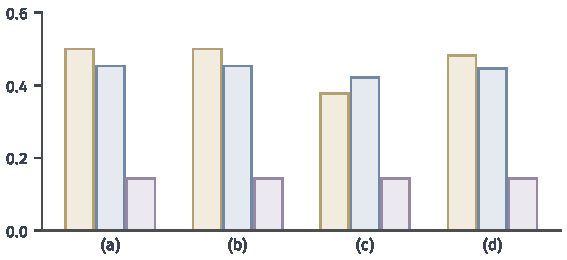
\includegraphics[width=96mm]{figures/07-probability/04-distribution-analysis/matplotlib/dep-transform-bars/figure.pdf}
  \caption{标准二元高斯（$\rho=0.5$）在四种坐标变换下的三个量：(a)原坐标；(b)$Y\mapsto10Y$；(c)$(\mathrm{e}^{X},\mathrm{e}^{Y})$；(d)$(\Phi(X),\Phi(Y))$。黄柱为相关系数的绝对值，蓝柱为距离相关（$90\times90$个Gauss--Hermite加权节点数值计算，约$0.453$、$0.453$、$0.422$、$0.445$），紫柱为互信息（nat，均为$0.144$）。}
  \label{fig:dep-transform-bars}
\end{BookInlineFigure}


\section{HSIC}
\label{sec:dep-hsic}

距离协方差用一种特定的权重比较特征函数，并且只适用于欧氏空间。第~\ref{chap:distribution-comparison}章的MMD给了比较两个分布的另一种通用办法：把分布映成再生核Hilbert空间中的核均值，再量两个核均值的距离。独立性问的正是两个分布$P_{(X,Y)}$与$P_X\otimes P_Y$是否相同，只要在乘积空间上选一个核，就能直接用MMD比较它们。

先回顾所用的记号。$k$是$\mathcal{X}$上的正定核，$\mathcal{H}_k$是它的RKHS。对满足$\mathbb{E}_{P}\sqrt{k(X,X)}<\infty$的分布$P$，核均值$m_P\in\mathcal{H}_k$由
\[
  \mathbb{E}_{P}[g(X)]=\langle g,m_P\rangle_{\mathcal{H}_k},\qquad g\in\mathcal{H}_k
\]
确定，取值为$m_P(y)=\mathbb{E}_{P}[k(X,y)]$。两个分布的MMD是两个核均值之差的范数$\lVert m_P-m_Q\rVert_{\mathcal{H}_k}$，记为$\operatorname{MMD}_k(P,Q)$，它等于$\mathcal{H}_k$单位球上期望差的最大值，平方可以写成核期望
\begin{equation}
  \operatorname{MMD}_k^{2}(P,Q)=\mathbb{E}\,k(U,U')-2\,\mathbb{E}\,k(U,V)+\mathbb{E}\,k(V,V'),
  \label{eq:dep-mmd-recall}
\end{equation}
其中$U,U'\sim P$，$V,V'\sim Q$，四者相互独立。若$P\mapsto m_P$是单射，称$k$为特征核，这时MMD为零当且仅当两个分布相同；欧氏空间上固定带宽的高斯核是特征核。

\subsection{联合分布的核比较}
\label{sec:dep-hsic-kernel-comparison}

在$\mathcal{X}$上取核$k$，在$\mathcal{Y}$上取核$l$。乘积空间$\mathcal{X}\times\mathcal{Y}$上最自然的核是两者的乘积
\[
  \kappa\bigl((x,y),(x',y')\bigr)=k(x,x')\,l(y,y'),
\]
称为\term{乘积核}（product kernel）。它仍是正定核：其Gram矩阵是两个Gram矩阵的逐元素乘积，正定性由Schur乘积定理保证，可参考\BookChapterRef{chap:rkhs}{卷四第23章“再生核Hilbert空间”}。本节假定$k,l$可测且有界，相应的RKHS可分，于是$\kappa$也有界，任何分布的核均值都存在。

\begin{definition}[HSIC]
\label{def:dep-hsic}
在上述条件下，$X$与$Y$关于核$k,l$的\term{Hilbert--Schmidt独立性准则}（Hilbert--Schmidt independence criterion），简称HSIC，定义为
\begin{equation}
  \operatorname{HSIC}_{k,l}(X,Y)=\operatorname{MMD}_{\kappa}^{2}\bigl(P_{(X,Y)},\,P_X\otimes P_Y\bigr).
  \label{eq:dep-hsic-def}
\end{equation}
\end{definition}

图~\ref{fig:dep-hsic-embedding}是这个定义的示意：两个分布各被送到$\mathcal{H}_\kappa$中的一个点，HSIC是这两点距离的平方。边缘乘积的核均值是$m_{P_X}$与$m_{P_Y}$的张量积：对独立的$\tilde{X}\sim P_X$、$\tilde{Y}\sim P_Y$，期望分解为
\[
  \mathbb{E}\bigl[k(\tilde{X},x)\,l(\tilde{Y},y)\bigr]=m_{P_X}(x)\,m_{P_Y}(y).
\]

\begin{BookInlineFigure}
  \centering
  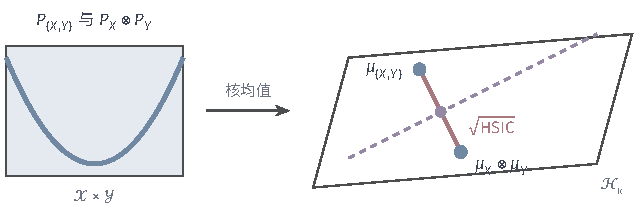
\includegraphics[width=107.9mm]{figures/07-probability/04-distribution-analysis/tikz/dep-hsic-embedding/figure.pdf}
  \caption{HSIC的几何图景。左：乘积空间上的两个分布，联合分布的质量集中在蓝色曲线上，边缘乘积摊在整个浅蓝矩形上。右：乘积核的RKHS$\mathcal{H}_\kappa$，两个核均值是两个蓝点，红色线段长度是$\sqrt{\operatorname{HSIC}}$。紫色虚线示意一个较贫乏的核只能看到的子空间：两个点在其上的投影（紫点）重合，这样的核给出零值。}
  \label{fig:dep-hsic-embedding}
\end{BookInlineFigure}

把式~\eqref{eq:dep-mmd-recall}用到这两个分布上，就得到只含核期望的表达。

\begin{theorem}[HSIC的核期望表示]
\label{thm:dep-hsic-expectation}
设$(X,Y)$、$(X',Y')$、$(X'',Y'')$相互独立且同分布。则
\begin{equation}
  \begin{aligned}
  \operatorname{HSIC}_{k,l}(X,Y)={}&\mathbb{E}\bigl[k(X,X')\,l(Y,Y')\bigr]+\mathbb{E}\bigl[k(X,X')\bigr]\,\mathbb{E}\bigl[l(Y,Y')\bigr]\\
  &-2\,\mathbb{E}\bigl[k(X,X')\,l(Y,Y'')\bigr].
  \end{aligned}
  \label{eq:dep-hsic-expectation}
\end{equation}
\end{theorem}

\begin{proof}
在式~\eqref{eq:dep-mmd-recall}中取$P=P_{(X,Y)}$，$Q=P_X\otimes P_Y$。第一项取$U=(X,Y)$，$U'=(X',Y')$，得$\mathbb{E}[k(X,X')l(Y,Y')]$。第三项中$V,V'$都服从边缘乘积，可以取$V=(X,Y'')$、$V'=(X',Y''')$，其中$Y'''$来自第四组独立复制；四个分量相互独立，期望分解为$\mathbb{E}[k(X,X')]\,\mathbb{E}[l(Y,Y')]$。第二项中$U=(X,Y)$，$V$服从边缘乘积且与$U$独立，取$V=(X',Y'')$，得到$\mathbb{E}[k(X,X')l(Y,Y'')]$。核有界，所有期望有限，代入即得。
\end{proof}

式~\eqref{eq:dep-hsic-expectation}与距离协方差的式~\eqref{eq:dep-dcov-pairwise}结构完全相同，只是把成对距离换成了核值。距离量的是“不相似”，核量的是“相似”，两者都在问：$X$这一对相似时，$Y$这一对是否也相似，超出边缘分布本身所能解释的程度。

\paragraph{中心化核}
与双重中心化同样，令
\[
  \tilde{k}(x,x')=k(x,x')-m_{P_X}(x)-m_{P_X}(x')+\mathbb{E}\,k(X,X'),
\]
称为\term{中心化核}（centered kernel），$\tilde{l}$类似。重复式~\eqref{eq:dep-dcov-centered}的验证（那里只用到中心化后对单个复制取期望为零），得到
\begin{equation}
  \operatorname{HSIC}_{k,l}(X,Y)=\mathbb{E}\bigl[\tilde{k}(X,X')\,\tilde{l}(Y,Y')\bigr].
  \label{eq:dep-hsic-centered}
\end{equation}
由再生性质展开可知，$\tilde{k}(x,x')$等于$k(x,\cdot)-m_{P_X}$与$k(x',\cdot)-m_{P_X}$在$\mathcal{H}_k$中的内积，就是把特征点平移到以核均值为原点后的内积。

\paragraph{交叉协方差算子}
HSIC这个名字来自另一种写法。对$f\in\mathcal{H}_k$、$g\in\mathcal{H}_l$，考虑$f(X)$与$g(Y)$的协方差。它对$f$、$g$都是线性的。由再生性质，$\lvert f(x)\rvert$不超过$\lVert f\rVert_{\mathcal{H}_k}\sqrt{k(x,x)}$，核有界时协方差被常数倍的$\lVert f\rVert\,\lVert g\rVert$控制。由Riesz表示定理，存在有界线性算子$\mathcal{C}_{XY}:\mathcal{H}_l\to\mathcal{H}_k$，使
\[
  \langle f,\mathcal{C}_{XY}\,g\rangle_{\mathcal{H}_k}=\operatorname{Cov}\bigl(f(X),g(Y)\bigr),
\]
称为\term{交叉协方差算子}（cross-covariance operator）。取$\mathcal{H}_k$与$\mathcal{H}_l$的规范正交基$\{e_i\}$、$\{e'_j\}$，HSIC等于这个算子的Hilbert--Schmidt范数的平方，
\begin{equation}
  \operatorname{HSIC}_{k,l}(X,Y)=\sum_{i,j}\operatorname{Cov}\bigl(e_i(X),\,e'_j(Y)\bigr)^{2}.
  \label{eq:dep-hsic-operator}
\end{equation}

式~\eqref{eq:dep-hsic-operator}可以从式~\eqref{eq:dep-hsic-centered}推出。记$\tilde{e}_i(x)=e_i(x)-\mathbb{E}e_i(X)$，由再生性质它等于$e_i$与$k(x,\cdot)-m_{P_X}$的内积。由Parseval等式，
\[
  \sum_i\tilde{e}_i(x)\,\tilde{e}_i(x')=\bigl\langle k(x,\cdot)-m_{P_X},\,k(x',\cdot)-m_{P_X}\bigr\rangle=\tilde{k}(x,x'),
\]
$\tilde{l}$同样展开。部分和由Cauchy--Schwarz不等式被$\lVert k(x,\cdot)-m_{P_X}\rVert\lVert k(x',\cdot)-m_{P_X}\rVert$控制，核有界时这是常数，可以用支配收敛定理交换求和与期望：
\[
  \mathbb{E}\bigl[\tilde{k}(X,X')\tilde{l}(Y,Y')\bigr]=\sum_{i,j}\mathbb{E}\bigl[\tilde{e}_i(X)\tilde{e}'_j(Y)\bigr]\,\mathbb{E}\bigl[\tilde{e}_i(X')\tilde{e}'_j(Y')\bigr].
\]
两组复制独立，每个乘积因子都是$\operatorname{Cov}(e_i(X),e'_j(Y))$，即得式~\eqref{eq:dep-hsic-operator}。

这个写法给出了直观：HSIC同时检查无穷多对特征函数$e_i(X)$、$e'_j(Y)$之间的协方差，把它们的平方加起来。协方差只检查一对线性函数；核越丰富，被检查的函数对越多。

\paragraph{线性核只剩协方差}
取最贫乏的核，$\mathcal{X}=\mathcal{Y}=\mathbb{R}$上的线性核$k(x,x')=xx'$、$l(y,y')=yy'$。它们无界，但当$X,Y$有二阶矩时式~\eqref{eq:dep-hsic-expectation}的各项仍然有限。代入，
\[
  \begin{aligned}
  &\mathbb{E}[XX'YY']+\mathbb{E}[XX']\,\mathbb{E}[YY']-2\,\mathbb{E}[XX'YY'']\\
  &\qquad=(\mathbb{E}XY)^{2}+(\mathbb{E}X)^{2}(\mathbb{E}Y)^{2}-2\,\mathbb{E}XY\,\mathbb{E}X\,\mathbb{E}Y ,
  \end{aligned}
\]
右边正是$\operatorname{Cov}(X,Y)^{2}$。线性核的RKHS只含线性函数，式~\eqref{eq:dep-hsic-operator}只剩一项。三点抛物线和连续抛物线在线性核下HSIC都是零。

\paragraph{距离诱导核}
距离协方差也是一个HSIC，只是用的核无界。在$\mathbb{R}^{d}$上令
\[
  k_{\mathrm{d}}(\bm{x},\bm{x}')=\tfrac12\bigl(\lVert\bm{x}\rVert_2+\lVert\bm{x}'\rVert_2-\lVert\bm{x}-\bm{x}'\rVert_2\bigr),
\]
称为\term{距离诱导核}（distance-induced kernel）。

它是正定的。由引理~\ref{lem:dep-cos-integral}，$k_{\mathrm{d}}$的三项各写成$1-\cos$的积分。记$\alpha=\langle\bm{t},\bm{x}\rangle$，$\beta=\langle\bm{t},\bm{x}'\rangle$，展开右边的乘积可以验证
\[
  \begin{aligned}
  &(1-\cos\alpha)+(1-\cos\beta)-\bigl(1-\cos(\alpha-\beta)\bigr)\\
  &\qquad=\operatorname{Re}\bigl[(\mathrm{e}^{\mathrm{i}\alpha}-1)\,\overline{(\mathrm{e}^{\mathrm{i}\beta}-1)}\bigr].
  \end{aligned}
\]
记
\[
  g_{\bm{x}}(\bm{t})=\mathrm{e}^{\mathrm{i}\langle\bm{t},\bm{x}\rangle}-1 .
\]

把三项的积分合并，得到
\[
  k_{\mathrm{d}}(\bm{x},\bm{x}')=\frac{1}{2c_d}\int_{\mathbb{R}^{d}}\frac{\operatorname{Re}\bigl[g_{\bm{x}}(\bm{t})\overline{g_{\bm{x}'}(\bm{t})}\bigr]}{\lVert\bm{t}\rVert_2^{d+1}}\,\mathrm{d}\bm{t},
\]
这是一个加权$L^{2}$内积的实部。对任意点$\bm{x}_1,\dots,\bm{x}_n$与实数$c_1,\dots,c_n$，
\[
  \sum_{i,j}c_ic_j\,k_{\mathrm{d}}(\bm{x}_i,\bm{x}_j)=\frac{1}{2c_d}\int_{\mathbb{R}^{d}}\frac{\bigl\lvert\sum_ic_ig_{\bm{x}_i}(\bm{t})\bigr\rvert^{2}}{\lVert\bm{t}\rVert_2^{d+1}}\,\mathrm{d}\bm{t}\geq0 .
\]

$k_{\mathrm{d}}$中的$\lVert\bm{x}\rVert_2$与$\lVert\bm{x}'\rVert_2$只依赖一个端点，在中心化中被消去，所以$\tilde{k}_{\mathrm{d}}=-\frac12A$，$A$是式~\eqref{eq:dep-double-centering}的双重中心化距离。代入式~\eqref{eq:dep-hsic-centered}与式~\eqref{eq:dep-dcov-centered}，在二阶矩有限时
\[
  \operatorname{HSIC}_{k_{\mathrm{d}},l_{\mathrm{d}}}(\bm{X},\bm{Y})=\tfrac14\operatorname{dCov}^{2}(\bm{X},\bm{Y}).
\]
距离协方差因此是HSIC的一个特例。核无界时，HSIC的每一项能否积分要另外检查，这里所需的正是二阶矩。

\paragraph{两个手算例子}
标准二元高斯在高斯核下有闭式。取$k(x,x')=\exp(-(x-x')^{2}/2)$，$l$相同（带宽$1$）。式~\eqref{eq:dep-hsic-expectation}的每一项都形如$\mathbb{E}\exp(-\frac12(U^{2}+V^{2}))$，其中$(U,V)$是均值为零的二元高斯，协方差矩阵记为$\bm{S}$。把高斯密度代入并配方，
\[
  \mathbb{E}\exp\Bigl(-\tfrac12(U^{2}+V^{2})\Bigr)=\frac{1}{2\pi\sqrt{\det\bm{S}}}\int_{\mathbb{R}^{2}}\mathrm{e}^{-\frac12\bm{w}^{\top}(\bm{S}^{-1}+\bm{I})\bm{w}}\,\mathrm{d}\bm{w}=\det(\bm{I}+\bm{S})^{-1/2}.
\]
三项分别对应$(U,V)=(X-X',Y-Y')$、两者独立、$(X-X',Y-Y'')$，协方差矩阵的对角元都是$2$，非对角元分别为$2\rho$、$0$、$\rho$。$\det(\bm{I}+\bm{S})$依次为$9-4\rho^{2}$、$9$、$9-\rho^{2}$，于是
\begin{equation}
  \operatorname{HSIC}=\frac{1}{\sqrt{9-4\rho^{2}}}+\frac13-\frac{2}{\sqrt{9-\rho^{2}}}.
  \label{eq:dep-hsic-gauss}
\end{equation}
$\rho=0.5$时三项为$0.35355$、$0.33333$、$-0.67612$，
\[
  \operatorname{HSIC}\approx0.35355+0.33333-0.67612=0.01076 .
\]

三点抛物线在同样的核下是有限和。记$\alpha=\mathrm{e}^{-1/2}\approx0.6065$，$\beta=\mathrm{e}^{-2}\approx0.1353$，三个点按$x=-1,0,1$排列，核矩阵为
\[
  \bm{K}=\begin{pmatrix}1&\alpha&\beta\\ \alpha&1&\alpha\\ \beta&\alpha&1\end{pmatrix},\qquad
  \bm{L}=\begin{pmatrix}1&\alpha&1\\ \alpha&1&\alpha\\ 1&\alpha&1\end{pmatrix}.
\]
式~\eqref{eq:dep-hsic-expectation}的三项分别是$\frac19\sum_{i,j}K_{i,j}L_{i,j}$、两个矩阵各自的元素平均之积、以及$\frac13\sum_i\bar{K}_i\bar{L}_i$（$\bar{K}_i,\bar{L}_i$为第$i$行的平均）。数值为
\[
  \begin{gathered}
  \mathbb{E}[kl]\approx0.52691,\qquad \mathbb{E}[kl'']\approx0.51771,\\
  \mathbb{E}[k]\,\mathbb{E}[l]\approx0.63298\times0.82512\approx0.52228,
  \end{gathered}
\]
所以$\operatorname{HSIC}\approx0.52691+0.52228-2\times0.51771\approx0.01378$。

\subsection{零值判据与核选择}
\label{sec:dep-hsic-zero}

由定义~\ref{def:dep-hsic}，HSIC为零当且仅当两个核均值相同。核均值能否分辨$P_{(X,Y)}$与$P_X\otimes P_Y$，取决于乘积核$\kappa$。

\begin{theorem}[HSIC的零值判据]
\label{thm:dep-hsic-zero}
若乘积核$\kappa=k\otimes l$在$\mathcal{X}\times\mathcal{Y}$的概率分布上是特征核，则
\begin{equation}
  \operatorname{HSIC}_{k,l}(X,Y)=0\iff X\text{与}Y\text{独立}.
  \label{eq:dep-hsic-zero}
\end{equation}
特别地，$\mathcal{X}=\mathbb{R}^{p}$、$\mathcal{Y}=\mathbb{R}^{q}$，$k,l$为带宽$\sigma,\tau>0$的高斯核时，结论成立。
\end{theorem}

\begin{proof}
式~\eqref{eq:dep-hsic-zero}是特征核的定义：MMD为零当且仅当两个分布相同。对高斯核，乘积核为
\[
  \kappa\bigl((\bm{x},\bm{y}),(\bm{x}',\bm{y}')\bigr)=\exp\Bigl(-\frac{\lVert\bm{x}-\bm{x}'\rVert_2^{2}}{2\sigma^{2}}-\frac{\lVert\bm{y}-\bm{y}'\rVert_2^{2}}{2\tau^{2}}\Bigr).
\]
作线性变换$T(\bm{x},\bm{y})=(\bm{x}/\sigma,\bm{y}/\tau)$，则$\kappa(\bm{z},\bm{z}')=k_1(T\bm{z},T\bm{z}')$，$k_1$是$\mathbb{R}^{p+q}$上带宽为$1$的高斯核。若两个分布$P,Q$的$\kappa$核均值相同，则推前分布$T_{\#}P$与$T_{\#}Q$的$k_1$核均值相同；$k_1$是特征核，所以$T_{\#}P=T_{\#}Q$，$T$可逆，于是$P=Q$。
\end{proof}

若$\sigma=\tau$，把第~\ref{chap:distribution-comparison}章高斯核MMD的谱表示用到$\mathbb{R}^{p+q}$上，HSIC就是$\lvert\Delta(\bm{t},\bm{s})\rvert^{2}$对高斯分布$\mathcal{N}(\bm{0},\sigma^{-2}\bm{I})$的积分。它与距离协方差的定义~\eqref{eq:dep-dcov-def}只差权重：高斯权重是可积的概率密度，不需要矩条件，但强烈压低高频；距离协方差的幂次权重不可积，换来了与距离的对应和尺度上的等变性。

特征核是充分条件。对欧氏空间上的平移不变核，已知只要$k$与$l$各自是特征核，HSIC的零值就刻画独立\scite{math-gretton2015hsic}。核不够丰富时，HSIC为零只说明它所检查的那些函数对的协方差都为零，例如线性核下只说明不相关。图~\ref{fig:dep-hsic-embedding}中紫色虚线表示的正是这种情况。

\paragraph{核尺度改变数值}
高斯核的带宽决定了HSIC“在多大尺度上看”。带宽很小时，核只在几乎重合的点对上取值接近$1$，连续分布下各项都趋于零；带宽很大时，在数据范围内$k(x,x')\approx1-(x-x')^{2}/(2\sigma^{2})$，核近似退化为常数加二次项，HSIC按$\sigma^{-4}$趋于零，并且主要反映协方差。中间某个尺度上HSIC最大。

图~\ref{fig:dep-hsic-bandwidth}对比两个分布：$\rho=0.5$的标准二元高斯（式~\eqref{eq:dep-hsic-gauss}的推广）与连续抛物线（数值积分），两个坐标用相同带宽$s$。抛物线的取值范围小，在$s\approx0.19$处达到最大值约$0.067$；高斯在$s\approx0.95$处达到约$0.0108$。两条曲线在$s\approx0.7$与$0.78$之间相交：带宽小于此时抛物线的HSIC更大，大于此时高斯的更大。$s=1$时两者分别为$0.0108$与$0.0026$。

\begin{BookInlineFigure}
  \centering
  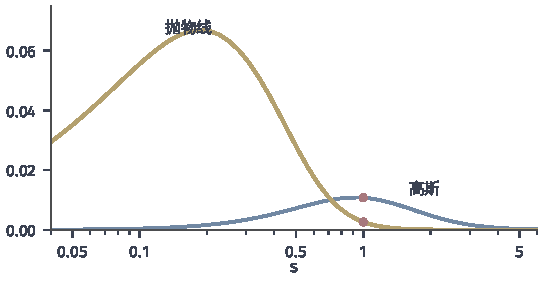
\includegraphics[width=92mm]{figures/07-probability/04-distribution-analysis/matplotlib/dep-hsic-bandwidth/figure.pdf}
  \caption{高斯核HSIC随带宽$s$的变化（横轴为对数刻度，两个坐标用同一带宽）。蓝线：$\rho=0.5$的标准二元高斯，闭式计算；黄线：$X\sim\operatorname{Unif}(-1,1)$、$Y=X^{2}$，对$X$取$1000$个节点数值积分。红点为$s=1$处的$0.0108$与$0.0026$。两条曲线在$s\approx0.74$附近相交。}
  \label{fig:dep-hsic-bandwidth}
\end{BookInlineFigure}

所以“这个分布的HSIC比那个大”只有在指定了核与带宽以后才有意义；换一个带宽，次序可以颠倒。不同核下的HSIC数值不在同一个刻度上，不能直接比较。把HSIC除以$\sqrt{\operatorname{HSIC}_{k,k}(X,X)\operatorname{HSIC}_{l,l}(Y,Y)}$可以得到与距离相关类似的归一化量，它消去了一部分尺度影响，但仍依赖带宽。根据样本选带宽的经验规则涉及估计问题，不在本章讨论。


\section{离散化评分}
\label{sec:dep-discretization}

还有一种更朴素的做法：把$X$的取值范围切成几段，$Y$的也切成几段，数一数每个格子里的概率，得到一张有限的概率表，再看这张表离独立有多远。这相当于只在给定的分辨率下观察两个变量。分辨率怎样选、选定以后丢掉了什么，是本节的问题。

设$\{\mathcal{A}_1,\dots,\mathcal{A}_k\}$是$\mathcal{X}$的有限可测划分，$\{\mathcal{B}_1,\dots,\mathcal{B}_l\}$是$\mathcal{Y}$的有限可测划分。记$\alpha(X)$为$X$所在的格子编号，$\beta(Y)$同理。格子标签的联合概率表为
\[
  p_{i,j}=\mathbb{P}\bigl(X\in\mathcal{A}_i,\ Y\in\mathcal{B}_j\bigr),\qquad i=1,\dots,k,\ j=1,\dots,l .
\]
这是一个总体对象：它由联合分布与选定的划分完全确定，与样本无关。

\subsection{固定划分的关联}
\label{sec:dep-fixed-partition}

对格子标签可以用任何离散的依赖度量，最自然的是它们的互信息$I(\alpha(X);\beta(Y))$。$\alpha,\beta$是可测函数，由定理~\ref{thm:dep-mi-invariance}，
\begin{equation}
  I\bigl(\alpha(X);\beta(Y)\bigr)\leq I(X;Y).
  \label{eq:dep-binned-mi-bound}
\end{equation}
离散化只会丢失信息。若一个划分细分了另一个划分，粗格子的标签是细格子标签的函数，再用一次同样的不等式，细划分的互信息不小于粗划分的。

\paragraph{零关联不能反推独立}
固定一个划分得到零互信息，只说明这张表上看不到依赖。连续抛物线$X\sim\operatorname{Unif}(-1,1)$，$Y=X^{2}$给出了反例。在$x=0$处切开$X$，在$y=1/4$处切开$Y$，这是两个边缘各自的中位数。四个格子的概率都可以直接算出：$\{X<0,\,Y<1/4\}=\{-1/2<X<0\}$，概率为$1/4$；其余三个同理，于是
\[
  p_{i,j}=\tfrac14=\tfrac12\cdot\tfrac12,\qquad i,j=1,2 .
\]
这张表恰好是独立的，格子标签的互信息为零，而$X$与$Y$并不独立。原因是$Y$只依赖$\lvert X\rvert$，而$X$的符号与$\lvert X\rvert$独立；在$x=0$处切开，记录的恰好是与$Y$无关的那部分信息。

把$X$的划分加细为四段$[-1,-\frac12)$、$[-\frac12,0)$、$[0,\frac12)$、$[\frac12,1]$，$Y$的划分不变。这时$Y$的格子标签由$X$的格子标签确定：$X$在中间两段时$Y<1/4$，在两端时$Y\geq1/4$。所以条件熵为零，
\[
  I\bigl(\alpha(X);\beta(Y)\bigr)=H\bigl(\beta(Y)\bigr)=\ln2\approx0.693 .
\]
图~\ref{fig:dep-partition-grids}画出这两个划分：同一条抛物线，粗划分下格子概率全为$1/4$，细划分下有四个格子为零。

\begin{BookInlineFigure}
  \centering
  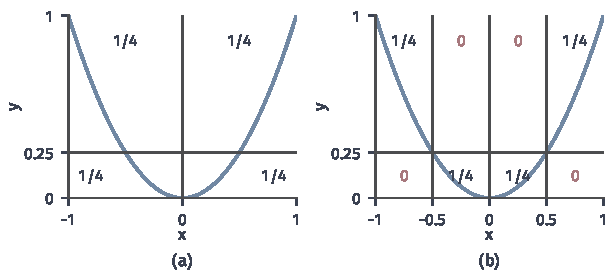
\includegraphics[width=104mm]{figures/07-probability/04-distribution-analysis/matplotlib/dep-partition-grids/figure.pdf}
  \caption{连续抛物线$y=x^{2}$（蓝）在两个固定划分下的格子概率（深灰线为格子边界）。(a)在$x=0$与$y=1/4$处切开，四个格子概率都是$1/4$，标签互信息为$0$；(b)$X$再在$\pm1/2$处切开，八个格子中四个概率为$0$（红），标签互信息为$\ln2$。}
  \label{fig:dep-partition-grids}
\end{BookInlineFigure}

\paragraph{加细的极限}
沿着一列越来越细的划分，标签互信息单调不减，并且不超过$I(X;Y)$。若这列划分最终能分辨所有可测集（例如实轴上以二进端点逐次对分），标签互信息的极限就是$I(X;Y)$；更一般地，互信息等于所有有限划分上标签互信息的上确界\scite{math-cover2006information}。这给出了互信息的另一种读法，也说明了离散化是“从下方逼近”。

在两个边缘都按$k$个等概率区间切分（$k\times k$网格）时，两个例子表现完全不同。对$\rho=0.5$的标准二元高斯，$k=2$时四个格子由象限概率决定，
\[
  \mathbb{P}(X>0,\,Y>0)=\frac14+\frac{\arcsin\rho}{2\pi}=\frac14+\frac{1}{12}=\frac13,
\]
概率表为
\[
  \begin{pmatrix}1/3&1/6\\1/6&1/3\end{pmatrix},\qquad I_2=\tfrac23\ln\tfrac43+\tfrac13\ln\tfrac23\approx0.0566 .
\]
$k$增大时$I_k$迅速上升，$k=8$约为$0.127$，$k=32$约为$0.141$，逼近$0.144$。对连续抛物线，$X$的$k$个等概率区间长为$2/k$，$Y$的$k$个等概率区间对应$\lvert X\rvert$上长为$1/k$的区间。$k$为偶数时，每个$X$格子恰好覆盖两个$Y$格子，且在其中各占一半，所以
\[
  I_k=H\bigl(\beta(Y)\bigr)-H\bigl(\beta(Y)\mid\alpha(X)\bigr)=\ln k-\ln2=\ln\tfrac{k}{2}.
\]
它随$k$无界增长，与定理~\ref{thm:dep-mi-infinite}的无穷大一致；$k=2$给出$0$，正是上面的反例。图~\ref{fig:dep-binned-mi}画出这两条序列。

\begin{BookInlineFigure}
  \centering
  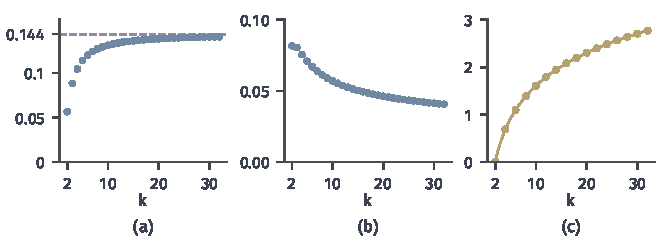
\includegraphics[width=112mm]{figures/07-probability/04-distribution-analysis/matplotlib/dep-binned-mi/figure.pdf}
  \caption{等概率$k\times k$网格上的标签互信息。(a)$\rho=0.5$的标准二元高斯，$I_k$（蓝点）单调上升，逼近紫色虚线$I=0.144$；(b)同一序列除以$\ln k$；(c)连续抛物线，$I_k=\ln(k/2)$（黄，偶数$k$；脚本对$k=4,8$另行数值核对），无界增长。}
  \label{fig:dep-binned-mi}
\end{BookInlineFigure}

\subsection{网格评分}
\label{sec:dep-grid-score}

固定的划分可能恰好错过依赖，自然的补救是在许多划分中搜索，取最能显示关联的那一个。可是互信息随格子数增长，格子越多越占便宜，比较不同大小的网格之前要先归一化。

对实值的$X,Y$，称把$X$的范围切成$k$个区间、$Y$切成$l$个区间所得的划分为一个$k\times l$网格$G$，标签互信息记为$I_G$。标签分别只有$k$与$l$种取值，所以
\[
  I_G\leq\min\bigl(H(\alpha(X)),H(\beta(Y))\bigr)\leq\ln\min(k,l).
\]
于是归一化的比值落在$[0,1]$中。给定格子预算$b\geq4$，定义总体的\term{网格评分}（grid score）
\begin{equation}
  S_b(X,Y)=\sup\Bigl\{\frac{I_G}{\ln\min(k,l)}:\ G\text{为}k\times l\text{网格},\ k,l\geq2,\ kl\leq b\Bigr\}.
  \label{eq:dep-grid-score}
\end{equation}
上确界取遍所有切点位置。令预算$b\to\infty$，得到的总体量就是Reshef等人的\term{最大信息系数}（maximal information coefficient），简称MIC\scite{math-reshef2016dependence}。

\paragraph{零值与确定关系}
总体网格评分的两端可以直接验证。若$X,Y$独立，每个网格的标签都独立，$I_G=0$，评分为零。反过来，若某个预算下评分为零，则所有$2\times2$网格的标签都独立；在$(a,c)$处切开的$2\times2$网格独立，意味着
\[
  \mathbb{P}(X\leq a,\,Y\leq c)=\mathbb{P}(X\leq a)\,\mathbb{P}(Y\leq c),
\]
它对一切$a,c$成立，联合分布函数分解，$X$与$Y$独立。所以只要允许任意切点，网格评分的零值也刻画独立；正是搜索弥补了单个固定划分的缺陷。

另一端，若$Y=f(X)$，$f$在有限个区间上分段连续且单调，$Y$的分布函数连续，则评分在足够大的预算下等于$1$。把$Y$按$l$个等概率区间切分，标签熵为$\ln l$；在单调段的端点与各$Y$切点的原像处切开$X$，每个$Y$格子的原像就是若干个$X$格子之并（对抛物线，取$X$的$2l$个区间即可），这时$Y$的标签由$X$的标签确定，$I_G=\ln l$，而$\min(k,l)=l$，比值为$1$。这与互信息给出$+\infty$形成对照：归一化把“确定关系”压到了上界$1$。

\paragraph{归一化与预算改变刻度}
评分的数值依赖于归一化规则和预算。图~\ref{fig:dep-binned-mi}(b)已经显示，对同一个高斯分布，等概率网格上的$I_k/\ln k$从$k=2$的$0.082$降到$k=32$的$0.041$：分子收敛到$0.144$，分母却继续增长。所以在不同的预算下、或者把分母换成$\ln k$或$\ln(kl)$，得到的是不同的刻度。MIC式的评分把高斯（$I=0.144$）放在$0$与$1$之间某处，把任意无噪声的函数关系都放在$1$，它衡量的是“网格能把关系捕捉得多完整”，不是信息量本身。

\paragraph{总体评分与经验评分}
实际使用时，评分是在一组样本上算的：用$n$个点的经验分布代替联合分布，在预算$b(n)$（常取$n^{0.6}$）以内搜索网格。这样得到的经验评分是另一个对象。即使两个变量独立，有限样本的经验表也不会恰好分解，经验互信息大于零；在许多网格上取最大值，又进一步把偏差放大。

图~\ref{fig:dep-grid-score-sample}用模拟说明这一点。为便于计算，这里只在等频网格中搜索，不优化切点位置，因此它低估了完整搜索的放大效应。对独立的均匀变量，$n=20$时经验评分的平均值约为$0.12$，$95\%$分位数约$0.28$；$n=2560$时平均值降到约$0.019$。对$Y=X^{2}+0.2Z$，$n=20$时经验评分的$5\%$分位数只有约$0.08$，低于独立变量的$95\%$分位数。小样本下两个分布的经验评分大量重叠：一个较高的经验分数，可能只是独立变量在有限样本上的波动。

\begin{BookInlineFigure}
  \centering
  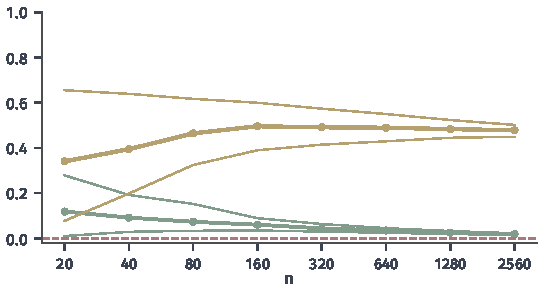
\includegraphics[width=92mm]{figures/07-probability/04-distribution-analysis/matplotlib/dep-grid-score-sample/figure.pdf}
  \caption{经验网格评分随样本量$n$的变化（横轴为对数刻度）。评分在$k,l\geq2$、$kl\leq n^{0.6}$的等频网格上取经验标签互信息除以$\ln\min(k,l)$的最大值。绿：独立的$\operatorname{Unif}(0,1)$对，总体评分为$0$（红色虚线）；黄：$X\sim\operatorname{Unif}(-1,1)$，$Y=X^{2}+0.2Z$。粗线为$200$次重复的平均，细线为$5\%$与$95\%$分位数。种子$719$。}
  \label{fig:dep-grid-score-sample}
\end{BookInlineFigure}

总体网格评分是联合分布的一个确定的泛函；经验评分是样本的函数，带有随机性和偏差。经验网格上的高分，不是“总体关系已经被可靠识别”的证明。要把经验分数变成关于总体的结论，需要分析它在独立假设下的分布并控制多次搜索带来的偏差，这是假设检验的任务，可参考\BookChapterRef{chap:confidence-sets-hypothesis-testing}{卷八第6章“置信集合与假设检验”}。


\section{度量的比较}
\label{sec:dep-comparison}

四类度量都从同一个问题出发：$P_{(X,Y)}$与$P_X\otimes P_Y$相差多少。它们在条件、零值、变换与刻度上的差别，决定了各自适合回答什么。

\paragraph{性质对照}
表~\ref{tab:dep-properties}把前面各节的结论放在一起。“零值刻画独立”一栏都是在所列条件下成立的；HSIC一栏指高斯核或其他使乘积核成为特征核的选择，线性核单独列出作为对照。

\begin{BookInlineTable}
  \centering
  \small
  \begin{tabular}{@{}p{15mm}p{22mm}p{13mm}p{26mm}p{20mm}@{}}
    \toprule
    度量 & 适用条件 & 零值刻画独立 & 保持不变的变换 & 取值与参数\\
    \midrule
    互信息 & 任意可测空间 & 是 & 双向可测一一映射 & $[0,\infty]$，无参数\\
    距离相关 & 欧氏空间，一阶矩 & 是 & 平移、正交、整体缩放 & $[0,1]$，无参数\\
    HSIC（高斯核） & 欧氏空间，无矩条件 & 是 & 平移、正交 & 非负，依赖带宽\\
    HSIC（线性核） & 实值，二阶矩 & 否 & 平移 & $\operatorname{Cov}^{2}$\\
    网格评分 & 实值，任意切点 & 是 & 严格增变换 & $[0,1]$，依赖预算\\
    \bottomrule
  \end{tabular}
  \caption{依赖度量的性质对照。“保持不变的变换”指对两个变量分别作该类变换时度量不变；HSIC在整体缩放下数值改变，除非带宽随之缩放。网格评分只依赖切点两侧的概率，严格增变换只移动切点，不改变可达到的概率表。}
  \label{tab:dep-properties}
\end{BookInlineTable}

表中的三列各自对应第一节的一件事。零值一栏回答“能否判断独立”，除线性核外答案都是肯定的，条件却不同：互信息不要求任何结构，距离相关要一阶矩，HSIC要合适的核，网格评分要求实值并允许任意切点。后两栏回答“非零数值有什么含义”，这里没有两种度量完全一致。

\paragraph{同一组分布上的数值}
表~\ref{tab:dep-values}列出本章几个例子的数值。互信息以nat为单位；HSIC用带宽为$1$的高斯核。

\begin{BookInlineTable}
  \centering
  \small
  \begin{tabular}{@{}lcccc@{}}
    \toprule
    联合分布 & 相关系数 & 互信息 & 距离相关 & HSIC\\
    \midrule
    三点抛物线 & $0$ & $0.637$ & $0.562$ & $0.0138$\\
    连续抛物线 & $0$ & $+\infty$ & $0.491$ & $0.0026$\\
    $Y=X^{2}+0.1Z$ & $0$ & $1.03$ & $0.461$ & $0.0026$\\
    高斯，$\rho=0.5$ & $0.5$ & $0.144$ & $0.454$ & $0.0108$\\
    高斯，$\rho=0.6$ & $0.6$ & $0.223$ & $0.550$ & $0.0166$\\
    \bottomrule
  \end{tabular}
  \caption{本章例子的依赖度量。连续抛物线与$Y=X^{2}+0.1Z$中$X\sim\operatorname{Unif}(-1,1)$，距离相关与HSIC由对$X$的数值积分得到；高斯的互信息由式~\eqref{eq:dep-gauss-mi}，距离相关由闭式，HSIC由式~\eqref{eq:dep-hsic-gauss}。}
  \label{tab:dep-values}
\end{BookInlineTable}

表中的相关系数在三个抛物线例子上都是零，其余三个度量都识别出了依赖。非零数值的次序则各不相同。比较$\rho=0.6$的高斯与$Y=X^{2}+0.1Z$：互信息说后者的依赖强得多（$1.03$对$0.223$），距离相关说前者更强（$0.550$对$0.461$）。图~\ref{fig:dep-ranking}画出这两个分布的样本。

\begin{BookInlineFigure}
  \centering
  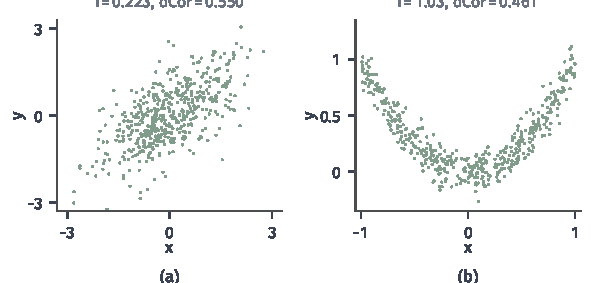
\includegraphics[width=100mm]{figures/07-probability/04-distribution-analysis/matplotlib/dep-ranking/figure.pdf}
  \caption{两个依赖度量给出相反次序的一对分布，各$500$个样本（绿，种子$719$）。(a)$\rho=0.6$的标准二元高斯；(b)$X\sim\operatorname{Unif}(-1,1)$，$Y=X^{2}+0.1Z$。图上方是总体互信息（nat）与距离相关：互信息认为(b)更强，距离相关认为(a)更强。}
  \label{fig:dep-ranking}
\end{BookInlineFigure}

两种判断都有道理，它们回答的是不同的问题。(b)中知道$X$以后，$Y$被限制在抛物线附近宽约$0.1$的窄带里，不确定性大幅减少，所以互信息大。但$X$的一对取值相距远时，$Y$的一对取值未必相距远：$X=\pm0.8$相距$1.6$，对应的$Y$几乎相同。距离相关问的是距离的同步，抛物线的折返削弱了这种同步，所以它更小。HSIC的次序还要看带宽：若两个坐标的带宽都取$1$，表~\ref{tab:dep-values}中高斯更大；若带宽取各坐标的标准差，(b)的HSIC约为$0.0286$，(a)约为$0.0166$，次序又与互信息一致。

\paragraph{真实值与可计算的下界}
互信息还有一个使用上的问题。连续抛物线的互信息是$+\infty$，$\sigma=0.1$的含噪抛物线是$1.03$，而数值方法得到的常常只是一个下界。第~\ref{chap:information-measures}章的InfoNCE下界在$N$个候选时不超过$\ln N$，候选数或评分函数的限制会让下界远低于真实值，并且对不同分布低估的程度不同。比较两个分布的互信息时，要比较的是真实值；拿两个下界的大小作比较，次序可能与真实值相反。

\paragraph{选择依赖度量}
没有一个度量能脱离任务给出统一的强度刻度。若关心的是一个变量能为另一个提供多少信息，且希望结果不受坐标和单位影响，用互信息，并准备好处理无穷大与估计困难。若变量是欧氏空间中的向量，希望用距离和有界的数值描述“取值是否一起变化”，用距离相关，并先统一各坐标的单位。

若变量取值于一般空间（文本、图、函数），或需要在特定尺度上检查依赖，用HSIC，并把核与带宽作为结论的一部分报告。若希望在给定分辨率下读出一张可解释的概率表，用离散化评分，并说明划分方式与归一化规则。几种量能同时判别独立，却可能给出不同的非零排序，选择之前先说清楚要比较的是哪一种依赖。


\section{本章小结}
\label{sec:dep-summary}

本章从$X\sim\operatorname{Unif}(-1,1)$与$Y=X^{2}$出发：协方差为零，依赖却是确定的。协方差只检查一对线性函数，独立要求联合分布等于边缘乘积，即对所有有界函数对乘积公式都成立。依赖度量就是对这一差别的量化，评价它时要分开三件事：零值是否刻画独立，非零数值随依赖怎样变化，以及能否从有限样本可靠判断。本章只讨论前两件。

互信息是联合分布相对边缘乘积的KL散度，零值在任何可测空间上刻画独立。它在双向可测的一一变换下不变，在不可逆的局部处理下不增，连续边缘时只依赖Copula。它不看取值之间的距离，也没有有限上界：在标准Borel空间上，只要$Y=f(X)$且$Y$的分布无原子，联合分布就集中在边缘乘积给零概率的图像上，互信息为无穷大。有限的计算下界不等于真实值。

距离协方差用权重$\lVert\bm{t}\rVert_2^{-(p+1)}\lVert\bm{s}\rVert_2^{-(q+1)}$对特征函数之差作平方积分。一阶矩保证它有限，零值由特征函数的唯一性刻画独立。二阶矩有限时它等于成对距离的三项期望，也等于双重中心化距离乘积的期望；中心化消去了只由边缘决定的部分，而指数$1$（不是$2$）使它看到非线性依赖。用距离方差归一化得到取值于$[0,1]$的距离相关，它在平移、正交变换和整体缩放下不变，取$1$当且仅当两组坐标只差一个相似变换，常量情形约定为$0$。

HSIC是联合分布与边缘乘积在乘积核下的平方MMD，等于核期望的三项组合，也等于交叉协方差算子的Hilbert--Schmidt范数平方。乘积核为特征核时零值刻画独立，高斯核满足这一条件；线性核只剩协方差的平方，距离诱导核给出距离协方差的四分之一。高斯核的带宽改变数值，甚至改变两个分布的次序。

离散化评分把取值装进有限个格子。固定划分的标签互信息不超过原互信息，可能恰好错过依赖；沿加细的划分它逼近互信息。在允许任意切点的网格中搜索并按$\ln\min(k,l)$归一化，总体评分的零值刻画实值变量的独立，分段单调的无噪声函数关系得分为$1$。经验网格评分是样本的函数，小样本下对独立变量也会给出明显的正值。

这些量能同时判别独立，却按不同的方式度量依赖：互信息量信息的减少，距离相关量距离的同步，HSIC量指定尺度上的特征协方差，网格评分量网格能否捕捉关系。选择之前要说清楚随机对象所在的空间、可积条件、需要保持的变换，并把零值判别与非零强度比较分开。用样本估计这些量、校准估计误差和检验独立性，由卷八的非参数推断与假设检验两章承接；算出一个样本分数，并不等于完成了统计判断。

